%%%%%%%%%%%%%%%%%%%%%%%%%%%%%%%%%%%%%%%%%
% Oliver Lemon made minor edits (jan 2015)  to : 
% Masters/Doctoral Thesis 
% LaTeX Template
% Version 1.43 (17/5/14)
%
% This template has been downloaded from:
% http://www.LaTeXTemplates.com
%
% Original authors:
% Steven Gunn 
% http://users.ecs.soton.ac.uk/srg/softwaretools/document/templates/
% and
% Sunil Patel
% http://www.sunilpatel.co.uk/thesis-template/
%
% License:
% CC BY-NC-SA 3.0 (http://creativecommons.org/licenses/by-nc-sa/3.0/)
%
% Note:
% Make sure to edit document variables in the Thesis.cls file
%
%%%%%%%%%%%%%%%%%%%%%%%%%%%%%%%%%%%%%%%%%

%----------------------------------------------------------------------------------------
%	PACKAGES AND OTHER DOCUMENT CONFIGURATIONS
%----------------------------------------------------------------------------------------

\documentclass[11pt, oneside]{Thesis} % The default font size and one-sided printing (no margin offsets)

\graphicspath{{Pictures/}} % Specifies the directory where pictures are stored

\usepackage[square, comma, sort&compress]{natbib} % Use the natbib reference package - read up on this to edit the reference style; if you want text (e.g. Smith et al., 2012) for the in-text references (instead of numbers), remove 'numbers' 
\hypersetup{urlcolor=blue, colorlinks=true} % Colors hyperlinks in blue - change to black if annoying
\usepackage{tabularx}
\usepackage[ruled,vlined]{algorithm2e}


\title{HWU CS Masters thesis template} % BUT you should use use " \title{\ttitle} " here instead to define the thesis title ! 
% \ttitle is defined in the file Thesis.cls 

\begin{document}

\frontmatter % Use roman page numbering style (i, ii, iii, iv...) for the pre-content pages

\setstretch{1.3} % Line spacing of 1.3

% Define the page headers using the FancyHdr package and set up for one-sided printing
\fancyhead{} % Clears all page headers and footers
\rhead{\thepage} % Sets the right side header to show the page number
\lhead{} % Clears the left side page header

\pagestyle{fancy} % Finally, use the "fancy" page style to implement the FancyHdr headers

\newcommand{\HRule}{\rule{\linewidth}{0.5mm}} % New command to make the lines in the title page

% PDF meta-data
\hypersetup{pdftitle={\ttitle}}
\hypersetup{pdfsubject=\subjectname}
\hypersetup{pdfauthor=\authornames}
\hypersetup{pdfkeywords=\keywordnames}

%----------------------------------------------------------------------------------------
%	TITLE PAGE
%----------------------------------------------------------------------------------------

\begin{titlepage}
\begin{center}

\textsc{\LARGE \univname}\\[1.5cm] % University name
\textsc{\Large Research Report}\\[0.5cm] % Thesis type

\HRule \\[0.4cm] % Horizontal line
{\huge \bfseries \ttitle}\\[0.4cm] % Thesis title
\HRule \\[1.5cm] % Horizontal line
 
\begin{minipage}{0.4\textwidth}
\begin{flushleft} \large
\emph{Author:}\\
\href{https://www.linkedin.com/in/noe-rivals/}{\authornames} % Author name - remove the \href bracket to remove the link
\end{flushleft}
\end{minipage}
\begin{minipage}{0.4\textwidth}
\begin{flushright} \large
\emph{Supervisor:} \\
{\supname} % Supervisor name - remove the \href bracket to remove the link  
\end{flushright}
\end{minipage}\\[3cm]
 
\large \textit{A thesis submitted in fulfilment of the requirements\\ for the degree of \degreename}\\[0.3cm] % University requirement text
\textit{in the}\\[0.4cm]
%\groupname\\

\deptname\\[2cm] % Research group name and department name
 
{\large \today}\\[1cm] % Date

\includegraphics[width=6cm]{./Figures/HWUlogo.jpg} % University/department logo - uncomment to place it
 
\vfill
\end{center}

\end{titlepage}

%----------------------------------------------------------------------------------------
%	DECLARATION PAGE
%	Your institution may give you a different text to place here
%----------------------------------------------------------------------------------------

\Declaration{

\addtocontents{toc}{\vspace{1em}} % Add a gap in the Contents, for aesthetics

I, \authornames, declare that this thesis titled, '\ttitle' and the work presented in it is my own. I confirm that this work submitted for assessment is my own and is
  expressed in my own words. Any uses made within it of the works of
  other authors in any form (e.g., ideas, equations, figures, text,
  tables, programs) are properly acknowledged at any point of their
  use. A list of the references employed is included.

%\begin{itemize} 
%\item[\tiny{$\blacksquare$}] This work was done wholly or mainly while in candidature for a research degree at this University.
%\item[\tiny{$\blacksquare$}] Where any part of this thesis has previously been submitted for a degree or any other qualification at %this University or any other institution, this has been clearly stated.
%\item[\tiny{$\blacksquare$}] Where I have consulted the published work of others, this is always clearly attributed.
%\item[\tiny{$\blacksquare$}] Where I have quoted from the work of others, the source is always given. With the exception of such %quotations, this thesis is entirely my own work.
%\item[\tiny{$\blacksquare$}] I have acknowledged all main sources of help.
%\item[\tiny{$\blacksquare$}] Where the thesis is based on work done by myself jointly with others, I have made clear exactly what %was done by others and what I have contributed myself.\\
%\end{itemize}
 \vspace{2cm} 
Signed:\\
\rule[1em]{25em}{0.5pt} % This prints a line for the signature

Date: 06/04/2021\\
\rule[1em]{25em}{0.5pt} % This prints a line to write the date
}

\clearpage % Start a new page

%----------------------------------------------------------------------------------------
%	QUOTATION PAGE
%----------------------------------------------------------------------------------------

\pagestyle{empty} % No headers or footers for the following pages

\null\vfill % Add some space to move the quote down the page a bit

\textit{``The first step is to establish that something is possible; then probability will occur."}

\begin{flushright}
Elon Musk
\end{flushright}

\vfill\vfill\vfill\vfill\vfill\vfill\null % Add some space at the bottom to position the quote just right

\clearpage % Start a new page

%----------------------------------------------------------------------------------------
%	ABSTRACT PAGE
%----------------------------------------------------------------------------------------

\addtotoc{Abstract} % Add the "Abstract" page entry to the Contents

%\abstract{\addtocontents{toc}{\vspace{1em}} % Add a gap in the Contents, for aesthetics

 {\huge{\textit{Abstract}} \par}{\addtocontents{toc}{\vspace{1em}} 
Imperfect game solving is an important field of research in AI. Research has been done on finding or approximating the equilibrium of a game. Once an equilibrium is found, the algorithm does not lose in the long term in a zero-sum game. Opponent exploitation is another approach to game solving, it tries to model the opponent's behavior and exploit it resulting in a higher reward. We will present a way of exploiting the opponent using neural network. We will evaluate our algorithm on the Kuhn poker variant. We will also explore its scalability for large information games with limit texas holdem poker.
%The page is kept centered vertically so can expand into the blank space above the title too\ldots
%

\clearpage % Start a new page

%----------------------------------------------------------------------------------------
%	ACKNOWLEDGEMENTS
%----------------------------------------------------------------------------------------

\setstretch{1.3} % Reset the line-spacing to 1.3 for body text (if it has changed)

\acknowledgements{\addtocontents{toc}{\vspace{1em}} % Add a gap in the Contents, for aesthetics

I would like to thank Dr. Michael Lones for supervising my project, giving me precious advice, and guiding me.
}
\clearpage % Start a new page

%----------------------------------------------------------------------------------------
%	LIST OF CONTENTS/FIGURES/TABLES PAGES
%----------------------------------------------------------------------------------------

\pagestyle{fancy} % The page style headers have been "empty" all this time, now use the "fancy" headers as defined before to bring them back

\lhead{\emph{Contents}} % Set the left side page header to "Contents"
\tableofcontents % Write out the Table of Contents

\lhead{\emph{List of Figures}} % Set the left side page header to "List of Figures"
\listoffigures % Write out the List of Figures

\lhead{\emph{List of Tables}} % Set the left side page header to "List of Tables"
\listoftables % Write out the List of Tables

%----------------------------------------------------------------------------------------
%	ABBREVIATIONS
%----------------------------------------------------------------------------------------

\clearpage % Start a new page

\setstretch{1.5} % Set the line spacing to 1.5, this makes the following tables easier to read

\lhead{\emph{Abbreviations}} % Set the left side page header to "Abbreviations"
\listofsymbols{ll} % Include a list of Abbreviations (a table of two columns)
{
\textbf{RNN} & \textbf{R}ecurrent \textbf{N}eural \textbf{N}etwork \\
\textbf{LSTM} & \textbf{L}ong \textbf{S}hort \textbf{M}emory \\
\textbf{EA} & \textbf{E}volutionary \textbf{A}lgorithms \\
\textbf{NN} & \textbf{N}eural \textbf{N}etwork \\
\textbf{CNN} & \textbf{C}onvolutional \textbf{N}eural \textbf{N}etwork
}

%----------------------------------------------------------------------------------------
%	PHYSICAL CONSTANTS/OTHER DEFINITIONS
%----------------------------------------------------------------------------------------

%\clearpage % Start a new page

%\lhead{\emph{Physical Constants}} % Set the left side page header to "Physical Constants"

%\listofconstants{lrcl} % Include a list of Physical Constants (a four column table)
%{
%Speed of Light & $c$ & $=$ & $2.997\ 924\ 58\times10^{8}\ \mbox{ms}^{-\mbox{s}}$ (exact)\\

%% Constant Name & Symbol & = & Constant Value (with units) \\
%}

%----------------------------------------------------------------------------------------
%	DEDICATION
%----------------------------------------------------------------------------------------

% \setstretch{1.3} % Return the line spacing back to 1.3

% \pagestyle{empty} % Page style needs to be empty for this page

% \dedicatory{For/Dedicated to/To my\ldots} % Dedication text

% \addtocontents{toc}{\vspace{2em}} % Add a gap in the Contents, for aesthetics

%----------------------------------------------------------------------------------------
%	THESIS CONTENT - CHAPTERS
%----------------------------------------------------------------------------------------

\mainmatter % Begin numeric (1,2,3...) page numbering

\pagestyle{fancy} % Return the page headers back to the "fancy" style

% Include the chapters of the thesis as separate files from the Chapters folder
% Uncomment the lines as you write the chapters

\chapter{Introduction} % Main chapter title

\lhead{Chapter 1. \emph{Introduction}} % This is for the header on each page - perhaps a shortened title

Imperfect game solving is the term used to solve a game where some information is unknown such as cards in poker. Imperfect game solving is an interesting field because it can be transposed easily to real-world problems. For example, in military, sometimes the opponent's resources are unknown or with a vague estimate, imperfect game solving algorithms are designed to handle state with unknown information.

Research in this field has been mostly focused on finding the equilibrium of a game. An equilibrium strategy played on the long term can not lose. It is the probabilistic solution to the game. On larger game state equilibrium can not be computed, algorithms are so trying to approximate it and get closer to it.

However, an equilibrium strategy does not guarantee the higher reward against an opponent. It just guarantees that on the long term, it will not lose. To improve the reward against an opponent, we need to exploit it. This is done by modeling the opponent's behavior and exploiting the mistakes made by him, this is called a sub-optimal opponent.

The problem is that whenever we try to exploit an opponent we are exposed to exploitability, this is referred to as the get-taught-and-exploited problem \citep{SANDHOLM2007382}. On another side, some research has proven that in some imperfect games, safe exploitation is possible introducing the notion of gift \citep{ganzfried2015safe}. Safe exploitation ensures that the opponent can be exploited without being exposed to exploitability. In this research we will not focused on having a safe exploitation, this is a choice made to fully explore the capacity of neural network and not limit it by the safe exploitation constraints.

Existing research has been done on opponent modeling in imperfect games. As said previously one demonstrates that safe opponent exploitation exists in some imperfect games such as poker \citep{ganzfried2015safe}, however, the method used in this paper do not scale for large game state or complex games. One research has been done for modeling large game state (poker limit texas hold'em) \citep{ganzfried2011game}. Both methods use a similar method. It uses a decision tree with a pre-computed equilibrium approximation, it plays a certain number of games against an opponent and updates the statistical difference between the equilibrium and the opponent choices. This difference defines the opponent model. This algorithm have multiple limitations. First, it requires playing a relatively high number of times against an opponent to start having a good result. Secondly in a large game tree, only the first branches will have an accurate opponent modeling, further we go in the tree less the algorithm has data. This is a major problem because it only models the opponent early game. Third, this method does not encode complex behavior, it is limited to the statistical mistake of the opponent. Fourth, it does not have a spatial representation, it means that the first or last game played by the opponent has the same weight in the opponent modeling. For example, it will not be able to model anger, opponent betting higher than usual after losing.

The goal of this project is to demonstrate that opponent modeling is possible with neural network and to assess the performances. We are aiming to have an algorithm that is not game-dependent and which is working with information that is available or computable for every imperfect game. This information is for example equilibrium and the game result. This will allow this algorithm to be re-used for other use cases.

We will at first works on a small game state to makes our experimentation. It would allow us to iterate faster and have rapid feedback on the architecture performance. We will use Kuhn poker which is an extremely simple version of poker \citep{kuhn1950simplified}. Then we will try to scale up the algorithm to a larger game state to assess the scalability. We will use limit texas holdem poker which has an info set size of \( 10^{14}\).

We will use recurrent neural network (RNN) because it will be able to use its output as input and so update the opponent model given the previous model. Recurrent neural network has proven to be able to learn complex problems. We are going to use another neural network to take actions within the game given the opponent model.

We will evaluate our model playing Kuhn poker. It will play against simple opponents that are easily exploitable and more advanced opponent that has already been exploited with other technique to have a comparison point. To evaluate the exploitability of our algorithm we will make it play against an equilibrium opponent. In addition, we will use the true best response algorithm that is known for exploitability testing \citep{johanson2011accelerating}.

This report is structured as follows:
\begin{itemize}
    \item \textbf{Chapter \ref{LR}, Literature Review}: This chapter covers the literature regarding machine learning models that had been considered for this project. It also explains the research made in imperfect game solving.
    \item \textbf{Chapter \ref{Methodology}, Methodology}: This chapter explains the architecture of the two neural networks, the methods that will be used to train them, and the evaluation process.
    \item \textbf{Chapter \ref{kuhn-poker}, Kuhn poker experiment}: This chapter details how the algorithm performed playing Kuhn poker and assess the potential of NN to model opponent.
    \item \textbf{Chapter \ref{scale-up}, Scale-up, limit texas holdem poker experiment}: This chapter explores the scalability of the algorithm by making it play limit texas holdem poker.
\end{itemize}

\chapter{Literature Review} \label{LR}

\lhead{Chapter 2. \emph{Literature Review}}
In this section, we will present multiple topics that have been studied to make the implementation choices.

The first sections will be dedicated to a general presentation of some machine learning model that has been considered for this project.

Then we will discuss the current state of the research about imperfect game solving. Presenting the different approaches to this problem.

\section{Machine learning models}
\subsection{Decision Tree}
Decision trees are a way of representing multiple choices and their outcome. As suggested by its name it uses a tree. The root node represents the initial state. Each link represents a decision, and the linked node is the outcome of this decision, usually represented by a new state.

This data structure is particularly useful to represent games. For example, a chess game can be represented by a decision tree where links are moved played and nodes the resulting game state. 

However, one major drawback of this data structure is that it can quickly become complex if there is an important depth (consecutive decision). For instance, for chess, it is impossible to represent a full decision tree because it contains too many different states. A common technique to overcome this limitation is to set a fixed depth and update the decision tree when it is traversed.

Metadata is often added to the link and the nodes to be processed easier by algorithms.

When decision trees are applied to games, an important notion is the Nash equilibrium \citep{nash1950equilibrium}. It represents the optimum decision to take for every state given the fact that the opponent is playing the best response. When a Nash Equilibrium is found for game, it is said that the game is solved. Given the actual computer limitation, such equilibrium can not be computed (or even stored) for complex games. In this case, algorithms try to approximate it, we will discuss it in more detail in section \ref{section:imperfect-game-solving:descision-tree}.

\subsection{Recurrent Neural Network} \label{LR:RNN}
Recurrent Neural Network (RNN) is a type of neural network that uses a part of its output for a part or all its input.

It is particularly interesting for his capacity to have an internal memory and remember the past input. A simple RNN is said to have a short memory and has been used for use-cases involving sequential data.

\subsubsection{LSTM} \label{LR:LSTM}
Long Short-Term Memory (LSTM) is a type of RNN that has increased the popularity of RNN by providing a long memory layout to the existing RNN. It has a specific design that allows having a way better space representation of the input and has proven to works well in many domains. In addition, it is also worth mentioning that it is by design opportune for creativity because it uses its output as input. For example, one project has been made to generate Game Of Throne book \citep{zackthoutt2017}. Or also generating music \citep{kotecha2018generating}.

Given its design, RNN can process and train on a large input given that it is a suitable input for RNN. Where other neural network architectures would not be able to works with it efficiently.

\subsection{Reinforcement Learning} \label{LR:reinforcement-learning}
\subsubsection{Overview}
Reinforcement Learning is a method used to train an algorithm based on experiences. An agent evolves in an environment, makes action, and learns from his mistake.

The basic idea is to have a reward given for an action or a set of actions. While learning the agent will try different actions and the reward will be used to update the algorithm. The update rules are specific to the algorithm used. It is common to use an extra formula to take into consideration the future expected reward.

While learning when the agent needs to take action, there is a set of methods that are common to all algorithms. It either \textbf{exploit}, take the best action (not necessarily optimal yet), or \textbf{explore}, pick a random action. A well-known method is epsilon greedy, it chooses to exploit or explore given predefined probability.

\subsubsection{Q-learning}

Q-learning \citep{watkins1992q} is a popular reinforcement learning method. It learns the Q-values, which are the expected reward of the actions given a state. The formula of a Q-value is: \(Q^{*}(s,a) = \max_{\pi}\sum \left [ r_{t} + yr_{t + 1} + y^{2}r_{t + 2} + ...|s_{t}=s,a_{t}=a, \pi \right ]\). Where \(a\) the the action, \(s\) is the state, \(\pi\) the policy and \(y\) the discount which represent how much the future reward should be take in consideration.

This formula has been limited to small state space due to its learning complexity. Recently research has been done to learn these Q-values with a large state space using neural network, it is Deep Q Network (DQN) \citep{mnih2015human}. This method uses another formula to compute the Q-values, making neural networks way more efficient to train. This method has proven to be successful, it has been used to makes an agent learn how to play 2600 Atari games using only the screen pixels for input \citep{bellemare2013arcade}.

DQN are only using the current state to take action, so it performs poorly when it requires the agent to remember the previous states. Research has been done to overcome this limitation combining DQN with Recurrent Neural Network (DRQN \citep{sorokin2015deep} \cite{chen2016deep}. Both of these methods use an attention system. \citep{chen2016deep} use an attention layer that takes all the previous state of the RNN and selects which information to take (figure \ref{fig:drqn-1}). On the other hand \citep{sorokin2015deep} use a part of the output of their RNN to define the next region of attention (figure \ref{fig:drqn-2}). On the figures you would notice that it is built with a CNN before, it is because these NN were designed to learn how to play Atari games from the screen pixels.

\begin{figure}[ht]
    \centering
    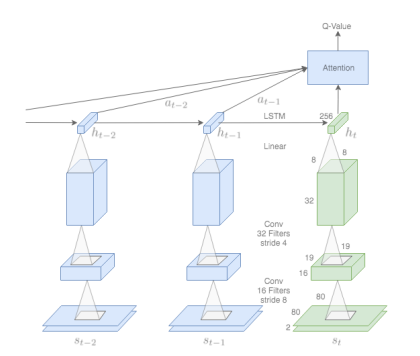
\includegraphics[width=0.7\textwidth]{Figures/drqn-1.png}
    \caption{DRQN with attention layer \citep{sorokin2015deep}}
    \label{fig:drqn-1}
\end{figure}

\begin{figure}[ht]
    \centering
    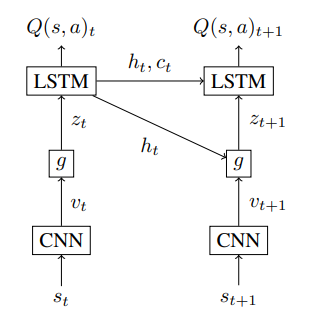
\includegraphics[width=0.5\textwidth]{Figures/drqn-2.png}
    \caption{DRQN with attention \citep{sorokin2015deep}}
    \label{fig:drqn-2}
\end{figure}

\subsection{Evolutionary Algorithms}
% TODO it could use a bit more in the evolutionary and co-evolutionary sections. For instance, a bit more intro to EAs, and maybe some discussion of any related problems co-evolution has been applied to (e.g. designing agents within particular environments, if you can find something like this)

\subsubsection{Overview}
Evolutionary algorithms are a wide category of AI. The idea is inspired by evolutionary biology and natural selection.

The main idea is to have multiple agents (population) evolving together. Each agent represents a potential solution. Agents are evaluated thanks to a fitness function, it defines how well an agent performed. They are evaluated, ranked, a new population is created then a selection is applied to the old generation. This process repeats until a solution is found.

There are multiple methods to perform the selection once the fitness has been calculated. The most commons are:
\begin{itemize}
    \item \textbf{Roulette Wheel Selection} (also called Fitness Proportionate Selection): the probability of selecting an individual is \(\frac{f_{i}}{\sum{f_{k}}} \). It can be represented as a wheel being spin to select the individual. \citep{golberg1989genetic}
    \item \textbf{Tournament Selection}: randomly take individuals from the population, take the best one of them \citep{goldberg1991comparative}
    \item \textbf{Ranked based Selection}: The fitness of the individuals is modified to their rank. For example, the worst individual gets a fitness of one, and the best individual a fitness equal to the population size. Then a roulette wheel selection is done with this new fitness. \citep{goldberg1991comparative}
\end{itemize}
In addition, all these methods have parameters that allow them to either apply more selective pressure or encourage diversity.

To create a new population, multiple methods can be used some may be specific to an EA category. First, an agent will inherit from one individual, all the data from an agent will be copied. From there you can apply mutation, randomly modifying a part of the data. The new agent can also inherit from multiple agents. In this case, there is a crossover/recombination, this mechanic is specific to the implementation of the EA. For example, a simple idea to inherit from two agents would be to take half of the data from one and half of the data from the other one. In addition, crossovers create a lot of diversity. However, if crossovers are made without much consideration it can lead to poor results, this is why there are often rules to guide the crossover.

Co-evolution is a notion we will rely on for this project. Co-evolution learning defines a way of calculating the fitness. It calculates the fitness based on the interaction between the individuals. So, the fitness is subjective and depends on the population. It is particularly useful the cases where a single fixed fitness function is difficult to establish. This differs from traditional EA.

\subsubsection{Collaborative co-evolution}

Collaborative co-evolution consists of evolving multiple agents working together to find a solution, each agent is a part of the solution.

Collaborative co-evolution has been studied for evolving neural network. One research worked on symbiotic adaptive neuro-evolution (SANE) system \citep{moriarty1997forming}. Instead of having each agent representing a neural network, neurons evolve together by being mixed up at every iteration (figure: \ref{fig:sane}). In addition, some neurons form symbiotic relationship, it means that they will likely be matched together in the same layout for the next generation.

\begin{figure}[ht]
    \centering
    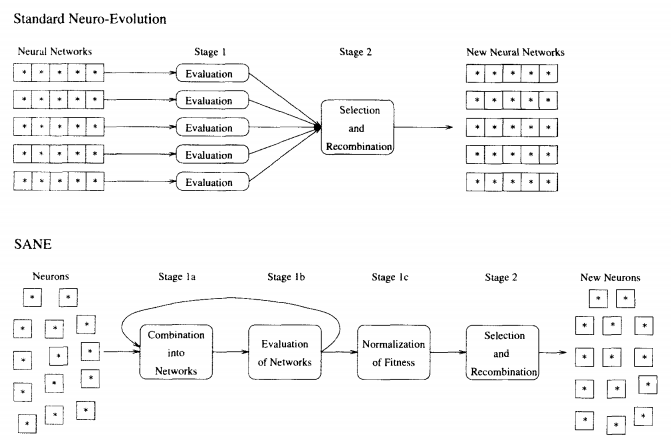
\includegraphics[width=0.85\textwidth]{Figures/sane.png}
    \caption{SANE method compared to Standard Neuro-Evolution \citep{moriarty1997forming}}
    \label{fig:sane}
\end{figure}

This co-evolution method helps to keep a high diversity and claim to have better performance and adaptation than standar elite/tournament method.

I think that such an algorithm is hard to setup, it requires a fine-tuning of the relations between neurons and how you create neural network with them. In addition, in nowadays development environment, such a method can lack performances compared to more supported algorithms.

\subsubsection{Competitive co-evolution} \label{LR:competitive-co-evolution}
Competitive co-evolution consists of multiple agents fighting together to have a higher reward. The fitness is directly based on the competition among the individuals.

One of the major problems of this technique is that it can quickly converge or and get stuck on a sub-optimal solution. In fact, if an agent happens to be stronger than the others then it will ultimately converge to it, even if it is a weak solution \citep{rosin1997new}. To reduce this effect, methods should be used to ensure diversity within the population and speed up the convergence to a perfect solution.

Teaching tests is a method that consists of injecting agents that have a fixed strategy. Those would help distinguish an optimal agent from a sub-optimal agent dominating the population \citep{rosin1997new}.

It is important to keep track of the previous agents, it would ensure that the algorithm is not making cycles and that future agents defeat the previous generation \citep{rosin1997new}. This can be done by injecting agents into the teaching set while training.

Fitness sharing is a method to promote diversity within the population. It is defined to take into account similarity between individuals and lower the fitness given the number of similarities. An idea is to consider each agent as a source of reward and that the reward needs to be shared among all individuals that defeat it. The fitness assigned to an agent is defined by \(\sum_{j \epsilon X}{\frac{1}{N_{j}}}\) where \(N_{j}\) is the number of agents defeating agent \(j\) and \(X\) is the population set \citep{rosin1997new}. Given this method, if a promising agent emerges and defeats an agent that only a few ones can defeat, it will likely be kept in the future generation. In addition, it reduces the convergence to a sub-optimal solution that exploits only a part of the population because the fitness will be divided.

\section{Imperfect game solving} \label{LR:section:imperfect-game-solving}
% TODO say that equilibrium finding if the main area of researsh
\subsection{Overview}
Imperfect game solving is an active field of research, this is a challenging topic for AI. It requires to deal with a high number of possibilities, this encourages to push the scalability limits of some AI models. In addition, it has to deal with unknown information. Furthermore, the evaluation process is tricky, there is no universal way to judge if one action is good or not. Usually, the evaluation is done by playing against other agents/individuals.

Imperfect game solving knowledge is not only about games. It is a way to use AI to works with unknown information. Real-world use cases often deal with unknown information, for example, finance, negotiation, strategic pricing, etc.

One of the most studied game in imperfect game solving is poker. This game has multiple advantages:
\begin{itemize}
    \item It has multiple variants from simple ones such as Kuhn poker to complex ones such as texas hold'em no limits.
    \item It has a wide community with a lot of professional players. This is an important point because the evaluation process may involve playing against professionals players with money, which makes the game results non-biased.
    \item Strategy matters, player choices have an important impact. A good agent playing poker against a weaker opponent will have a high chance to win.
    \item It is a complex game. Bluffing is an important part of the game and is a complex notion.
\end{itemize}

In the following section, we will discuss two main models used in imperfect game solving, Decision Tree and Neural Network. Then we will introduce the notion of exploitability.

\subsection{Decision Tree}
\label{section:imperfect-game-solving:descision-tree}
In imperfect game solving decision trees are widely use and most of the existing approaches use it.

Decision trees are tricky to build for imperfect games because to compute the outcome of a decision it requires to take into account all the possible hidden states.

Ultimately the Nash Equilibrium strategy does not care about hidden state because there is no information about it. An optimum action is given a known state. However, during the equilibrium solving or estimation, the hidden state must be used to estimate/calculate the reward.

For a medium/large game state, abstractions are made to limit the number of representations. For example, in poker, similar combinations of cards are grouped \citep{johanson2013evaluating}.

Successfully poker bot such as Libratus \citep{brown2018superhuman} or Baby Tartanian \citep{brown2016baby} estimates equilibrium on a large game state using MCCFR (Monte Carlo Counterfactual Regret Minimization). It is a reinforcement learning method consisting of playing against itself and updating the strategy based on how much the AI regrets not have selected an action in the past. This process is pre-computed for the first stages, then due to the complexity, it needs to be run in real-time.

Decision tree with equilibrium finding is nowadays the way that has proven to works the best for imperfect game solving.

\subsection{Neural Network}
Neural network has been used for imperfect game solving. We will present two use cases, one using supervised learning and the other one reinforcement learning.

One of the most successful uses of Neural Network in imperfect game solving is DeepStack \citep{moravvcik2017deepstack}, a poker bot. It uses neural network to approximate the opponent's counterfactual values and so decide which action to take (figure \ref{fig:deepstack}). One neural network is trained for each stage of the game, each one uses the output of the previous neural network as input. They trained these neural networks using supervised learning from randomly generated poker situations.

\begin{figure}[ht]
    \centering
    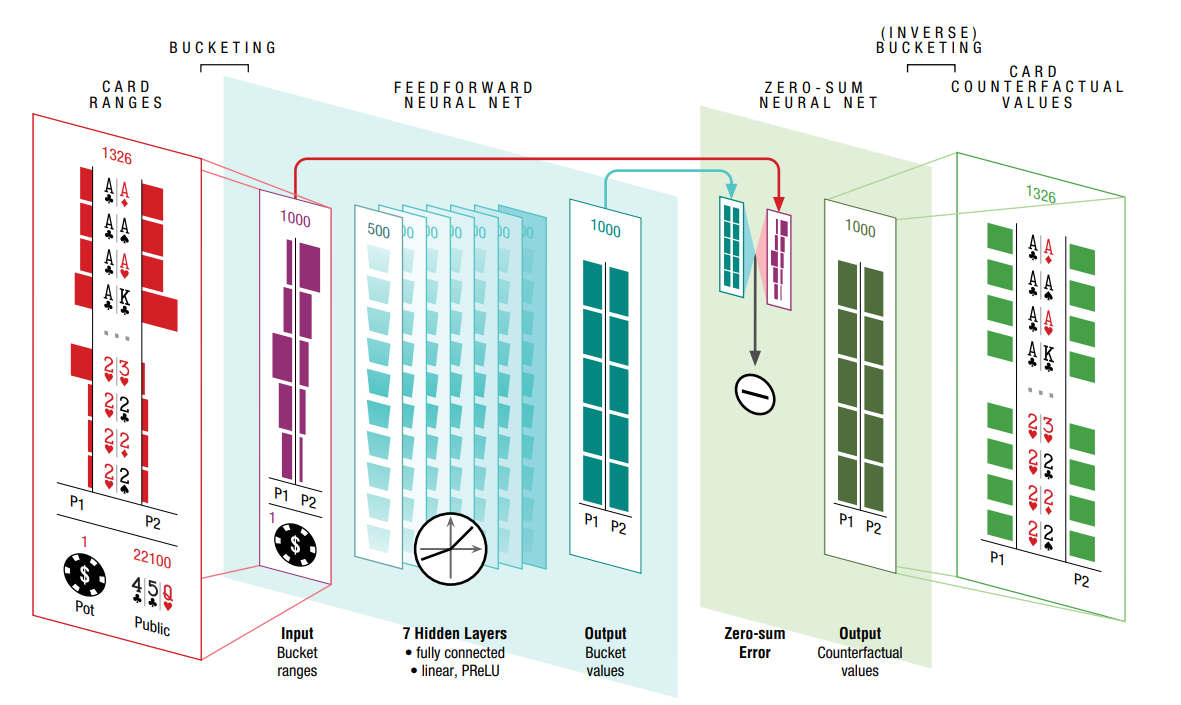
\includegraphics[width=1\textwidth]{Figures/deepstack.png}
    \caption{DeepStack counterfactual value network \citep{moravvcik2017deepstack}}
    \label{fig:deepstack}
\end{figure}

Rlcard \citep{zha2019rlcard} is an implementation of Deep-Q learning \citep{DBLP:journals/corr/MnihKSGAWR13} for imperfect game solving. It also uses NSFP (Neural Fictitious Self-Play) to manage the learning environment and DeepCFR to train the agent. The neural network is always fed with the same "info set" which is an absolute representation of the game. The idea is to bind an action to an info set thanks to neural network. It has proved that neural network and reinforcement learning can perform well in this area. In addition, this implementation is not specific to a game and can be applied to any imperfect game. On the other hand, due to this not specific implementation, it can not have abstraction. So, games with a large game state such as poker texas hold'em are not expected to have good performance.

\subsection{Exploitation in imperfect game solving}
Exploitation aims to identify and exploit the weaknesses of an opponent. Opponent modelling is the process of identifying the way the opponent is playing. If an opponent model is accurate exploiting it is straightforward.

Exploitation is a tricky process because it comes with exploitability. While deviating from the optimum to maximize the reward based on the previous action of the opponent there is a chance to be exploited. This is known as the "get taught and exploited problem" \citep{SANDHOLM2007382}.

It is called safe opponent exploitation when exploitation is done without possibility of being exploited and unsafe opponent exploitation when the possibility of being exploited is assumed.

\subsubsection{Unsafe opponent exploitation}
One research has been done on modelling the opponent in large information games \citep{ganzfried2011game}. They decided to assume that by exploiting an opponent they were going to be exposed to exploitation. They used an algorithm called Deviation-Based Best Response (DBBR), which statistically learns the deviation made by an opponent from an approximated equilibrium. In this way, it can exploit the statistical mistake made by an opponent.

One interesting thing about this research is that it relies on concepts available in every game, which is Nash-equilibrium and best response. This means that their method can be generalized to other imperfect games.

On the other hand, this algorithm has major issues, it requires to play a high number of games against an opponent to have a relatively good model. Even with that, the model will only be accurate in the early stages because it will not have enough sample of the opponent strategy in the middle/late. Indeed, decision trees are immense for imperfect games and it is unrealistic to have a usable model opponent for all the stages of the game with this algorithm.

The exploitation is also purely statistical, it can not model complex behavior. It also treats all the games with the same weight, it does not take an account the temporally of each game. For example, it would be impossible to model anger, the fact that if an opponent loses the previous game it will play aggressively the next one.

\subsubsection{Safe opponent exploitation}
Safe opponent exploitation is the idea of exploiting an opponent without the capacity of being exploited. It was stated that it was not possible \citep{ganzfried2011game}.

However, a recent research on safe opponent exploitation has proven that it was possible on some game \citep{ganzfried2015safe}. They introduce the notion of gift, profitable strategies that can be used by identifying sub-optimal opponent behavior. These gifts are defined formally for each game and can not be generalized.

Safe opponent exploitation relies heavily on equilibrium and plays the equilibrium strategy most of the time. During the evaluation process of this study, they played against dump agents, that for example always fold. It is hard to estimate how important does safe exploitation would make a difference with a more subtle sub-optimal agent.

The main issue with safe exploitation is that the extra reward from exploiting the opponent is limited by an important set of rules. In addition, the safe exploitation is game-specific and is impossible to generalize, it needs to be re-proven for each use case.

% TODO say somewhere that the game state size if equal to the info and action set size (or something like that)

\chapter{Methodology} \label{Methodology}

\lhead{Chapter 3. \emph{Methodology}}
In this section, we will cover the implementation details of this project.

First, we will discuss the different neural network architectures then we will discuss the training of these neural networks and finally how we are going to evaluate them.

We are assuming to know the equilibrium. It is a shortcut we are making because a lot of research had been done on equilibrium finding (section: \ref{LR:section:imperfect-game-solving}) and if we assume to know an equilibrium or a partial equilibrium this would help to reduce the input of the neural networks and improve the learning time.

We are aiming to have an algorithm that is universal to every imperfect game. To do so we are relying on notions that are common to all imperfect games, such as equilibrium and the reward of a game.

\section{Neural Network Architecture} \label{methodology:NN}
There will be two neural networks, one that builds the opponent model and one that decides which actions should be taken during a game. I have decided to use two NN because I believe that the opponent modeling NN requires to have the knowledge of a full game. In addition that will allow to have a specific set of information for the input of these NN and so improve the learning speed.

For optimization reasons, we do not want that these neural networks have to learn how the game works. Instead, we will try to process the input feed to these neural networks with the game knowledge. For example, giving the equilibrium of an action instead of giving the info set (the info set is the representation of the public and private information). It is a challenging constraint but we believe that it will enable this NN to scale way better.

\subsection{Opponent modelling NN} \label{methodology:opponent-modelling}
For the opponent modeling neural network, it needs to learn how the opponent play over time. To do that it needs to have multiple knowledge.

\subsubsection{Knowledge of previous games}

It needs to know previous games. It is done by having memory. Either an internal memory such as LSTM (section: \ref{LR:LSTM}) or by having a manual memory which is using information from the output of the neural network as its input. These kinds of neural networks are RNN (section: \ref{LR:RNN}).

\subsubsection{Knowledge about game history} \label{methodology:opponent-modelling:game-history}

It needs to know the game history. The game history consists of the multiple actions that had been done during a game. With a game history, you're supposed to be able to know every step of the game. A simple idea would be to give the different info set and the different actions taken by each player. However as said previously we do not want to feed the info set to the neural network.

Instead our idea is to represent the game history with a succession of:
\begin{itemize}
    \item agent action
    \item opponent action
    \item equilibrium for the opponent action
\end{itemize}

Like this, the game knowledge is encapsulated in the \textit{equilibrium for the opponent action}.

The equilibrium for an opponent's action is not always known. Indeed, to know it we need to have access to the private information of the opponent. In some cases, this information will not be known and we can not ignore this case.

One approach to this problem is to treat the two cases separately \citep{ganzfried2015safe}. However, because we are using a neural network the size and meaning of the input are rigid. That would require having two different neural networks. For the sake of simplicity and optimization reasons, we decide to not treat this.

One thing worth mentioning is that even if we do not know the private information of the opponent we can still use the equilibrium to give game knowledge. Indeed, instead of having a specific equilibrium for the information set, you can have a global equilibrium. For example in poker, if you're the first player you should bet 50\% of the time (the \% is just here, for example, it depends on the poker variant). So, if you notice that the opponent bet only 10\% of the time you can exploit it. It means that this global equilibrium is valuable information.

We decided to represent both of these equilibrium knowledge for the opponent's action. The global equilibrium and the specific equilibrium. If the private information of the opponent is unknown we can not have a specific equilibrium and so will just set the specific equilibrium values to -1 to indicate that no values are available. Figure \ref{fig:opponent-equilibrium}

\begin{figure}[ht]
    \centering
    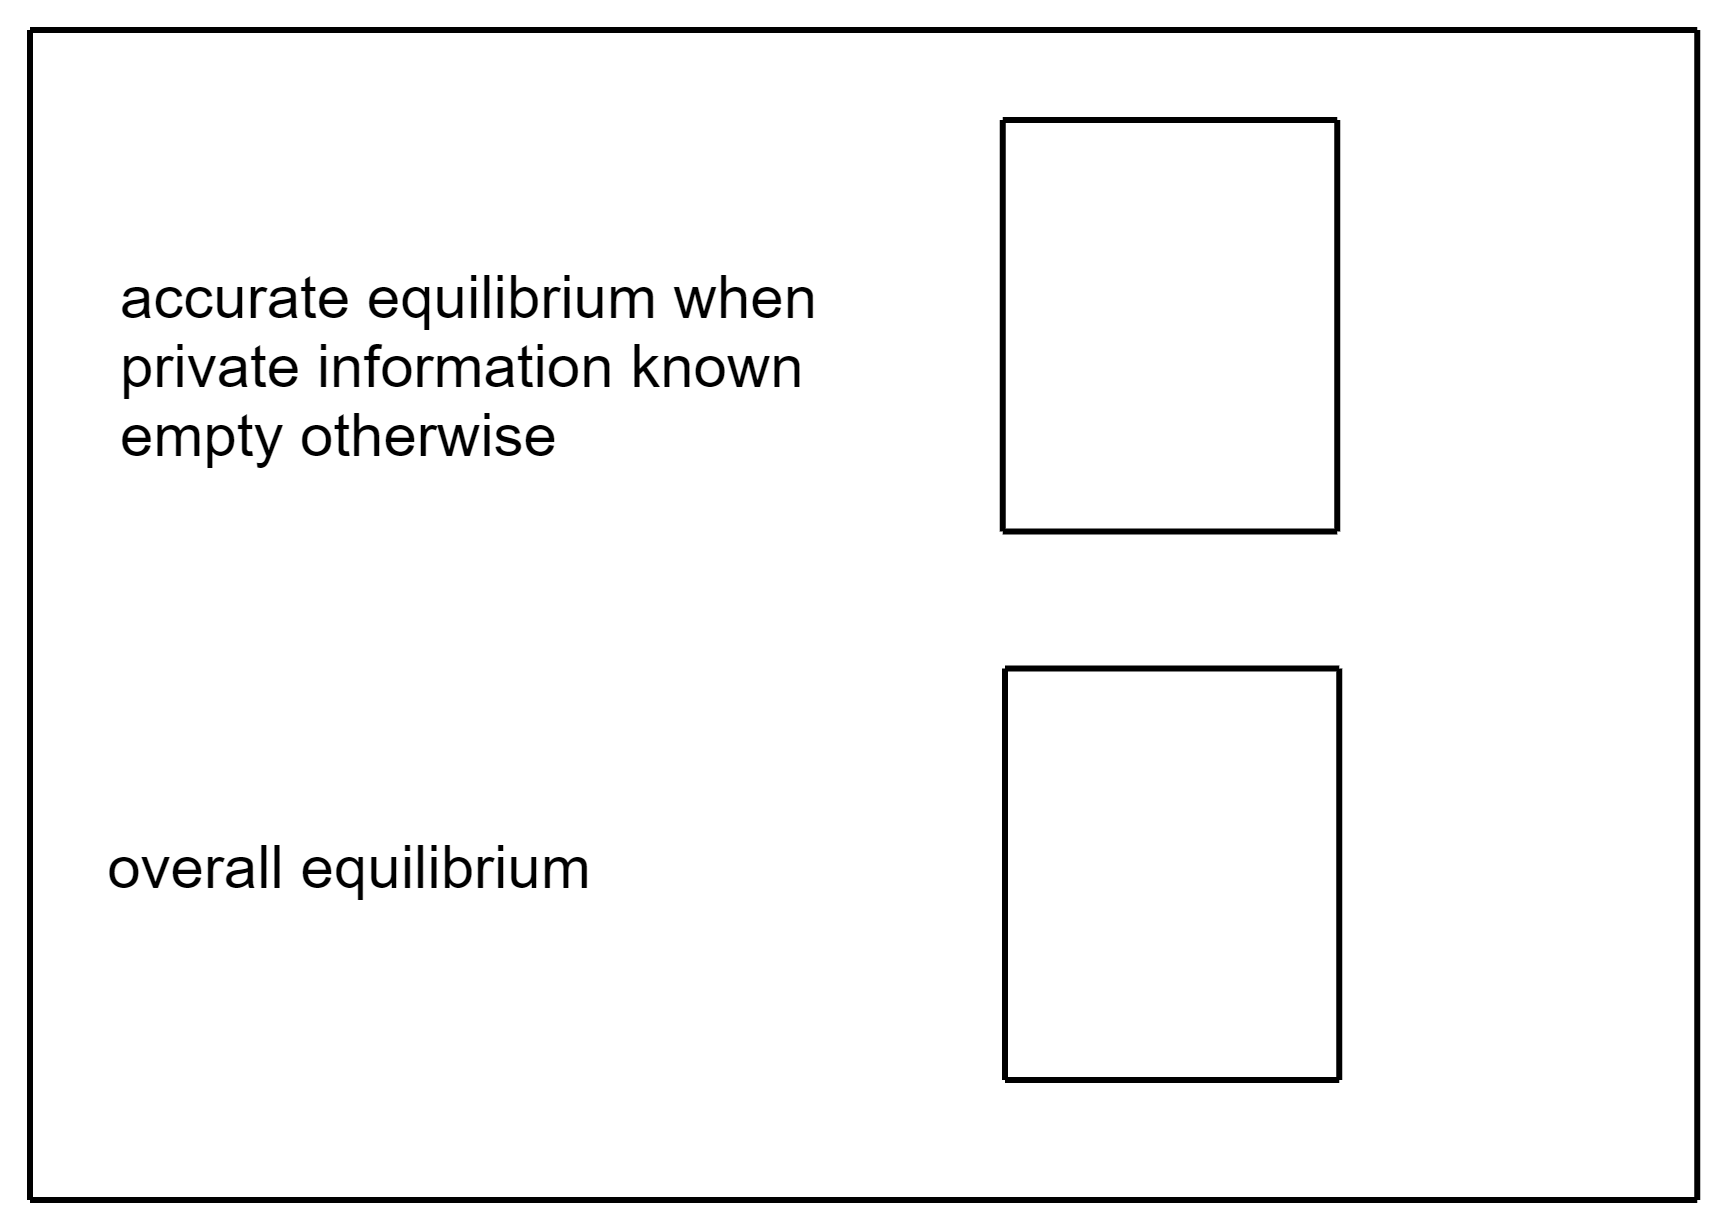
\includegraphics[width=0.7\textwidth]{Figures/opponent-equilibrium.png}
    \caption{Equilibrium for the opponent action}
    \label{fig:opponent-equilibrium}
\end{figure}

Also, another representation that we are thinking of is representing either the specific or the global equilibrium depending if we know the private information of the opponent. And to indicate the NN that it's the specific equilibrium we will have a flag (a binary value) set to 1 if it is the specific equilibrium.

Also to not mess up with the order of the input, if the opponent start we leave empty the first agent action.

Finally, because the input size of NN is constant we can not change the size of the input depending on the number of actions done in the game. To overcome this issue we will left empty a part of the input if the game stopped before.

\subsubsection{Knowledge about game result}

In the effort of feeding up the NN with game knowledge, we believe that the game result is valuable information that will greatly improve the performance of the NN.

The game result is as its name suggests the outcome of the game. For example in poker who won and how much money the player won.

This is the only part of the NN that is game-specific because each game can have valuable outcome information. However, we believe that it is not a problem for the generalization of this algorithm to other imperfect games. Indeed the outcome information is easy to retrieve and in most of the games, it only represents a small set of information.

\subsubsection{Conclusion}

In figure \ref{fig:opponent-modelling-nn-rnn} you can find a sum-up of this information with a RNN architecture where the opponent model also represents the NN memory. In figure \ref{fig:opponent-modelling-nn-lstm} it is the same information however the memory is managed internally as an LSTM would do.

\begin{figure}[ht]
    \centering
    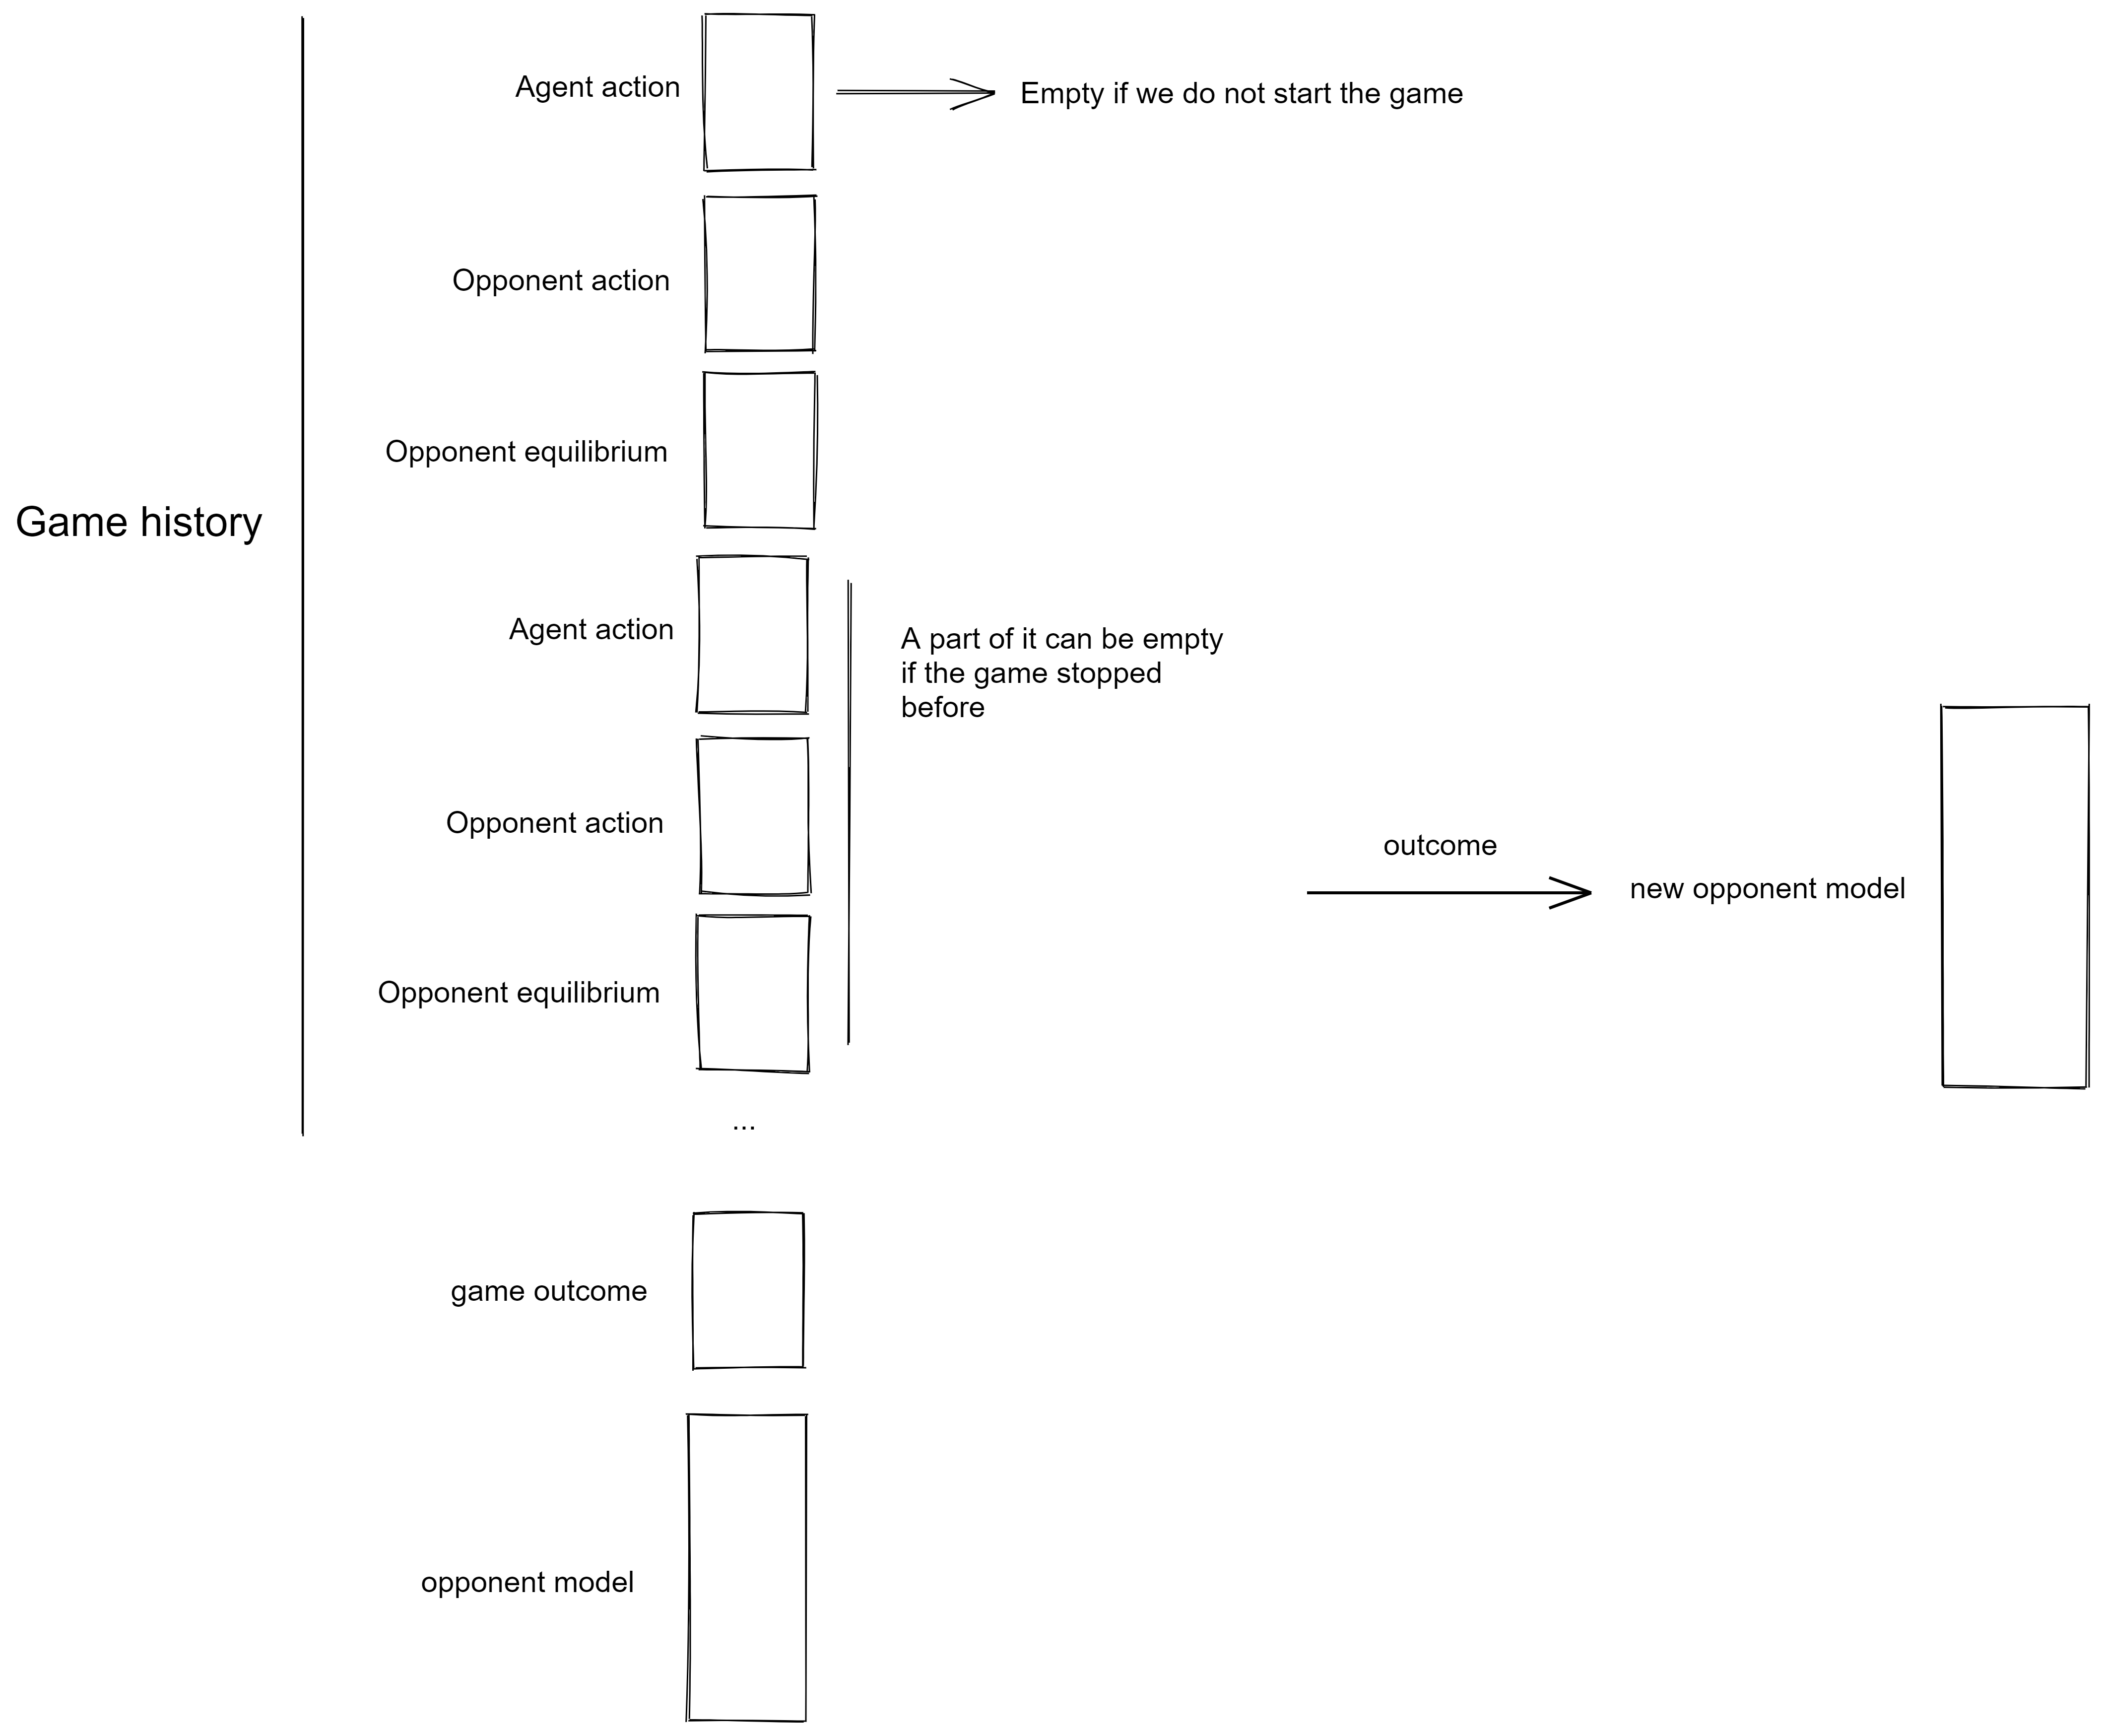
\includegraphics[width=0.9\textwidth]{Figures/opponent-modelling-nn-rnn.png}
    \caption{Opponent modelling neural network, simple RNN}
    \label{fig:opponent-modelling-nn-rnn}
\end{figure}

\begin{figure}[ht]
    \centering
    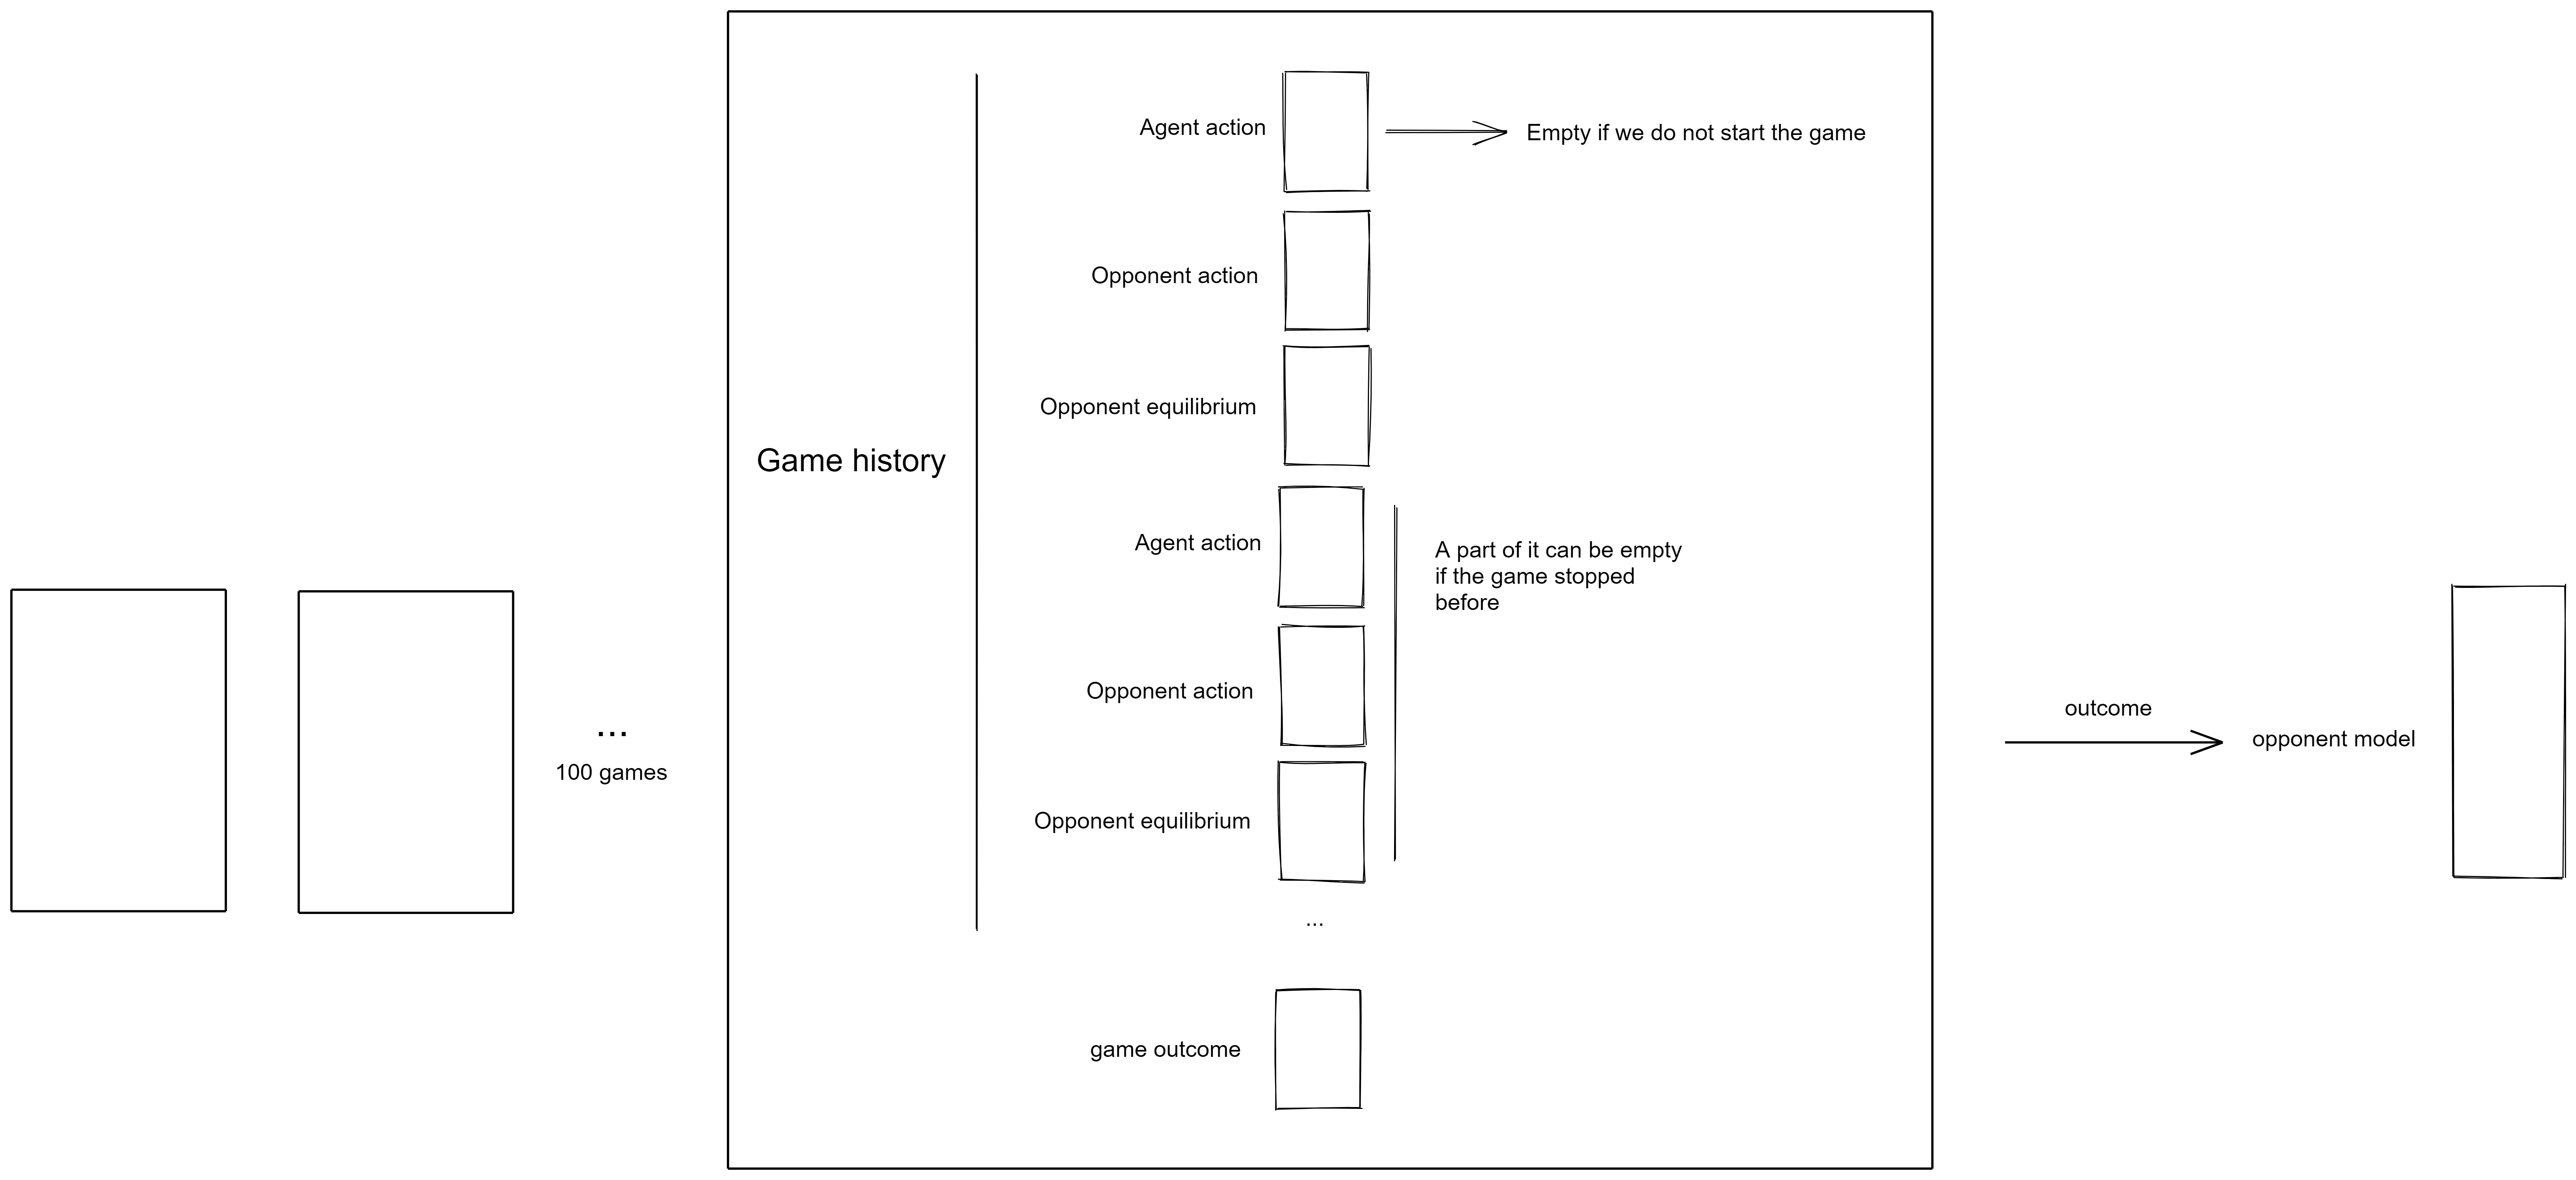
\includegraphics[width=1\textwidth]{Figures/opponent-modelling-nn-lstm.png}
    \caption{Opponent modelling neural network, LSTM kind}
    \label{fig:opponent-modelling-nn-lstm}
\end{figure}

\subsection{Decision making NN} \label{methodology:descision-making}
The decision-making NN is the one that will use the opponent model to decide which action to take within a game.

It needs to have information about the game history, we use the same representation as for the opponent modeling (section \ref{methodology:opponent-modelling:game-history}) however we do not add information about the opponent equilibrium. This might change if we see that including the global equilibrium for each agent action improve the performance.

In addition, we are giving the equilibrium of the current action for the agent. It continues the effort of feeding knowledge of the game to the NN.

You can find a schema of this neural network in figure \ref{fig:decision-making-nn}

\begin{figure}[ht]
    \centering
    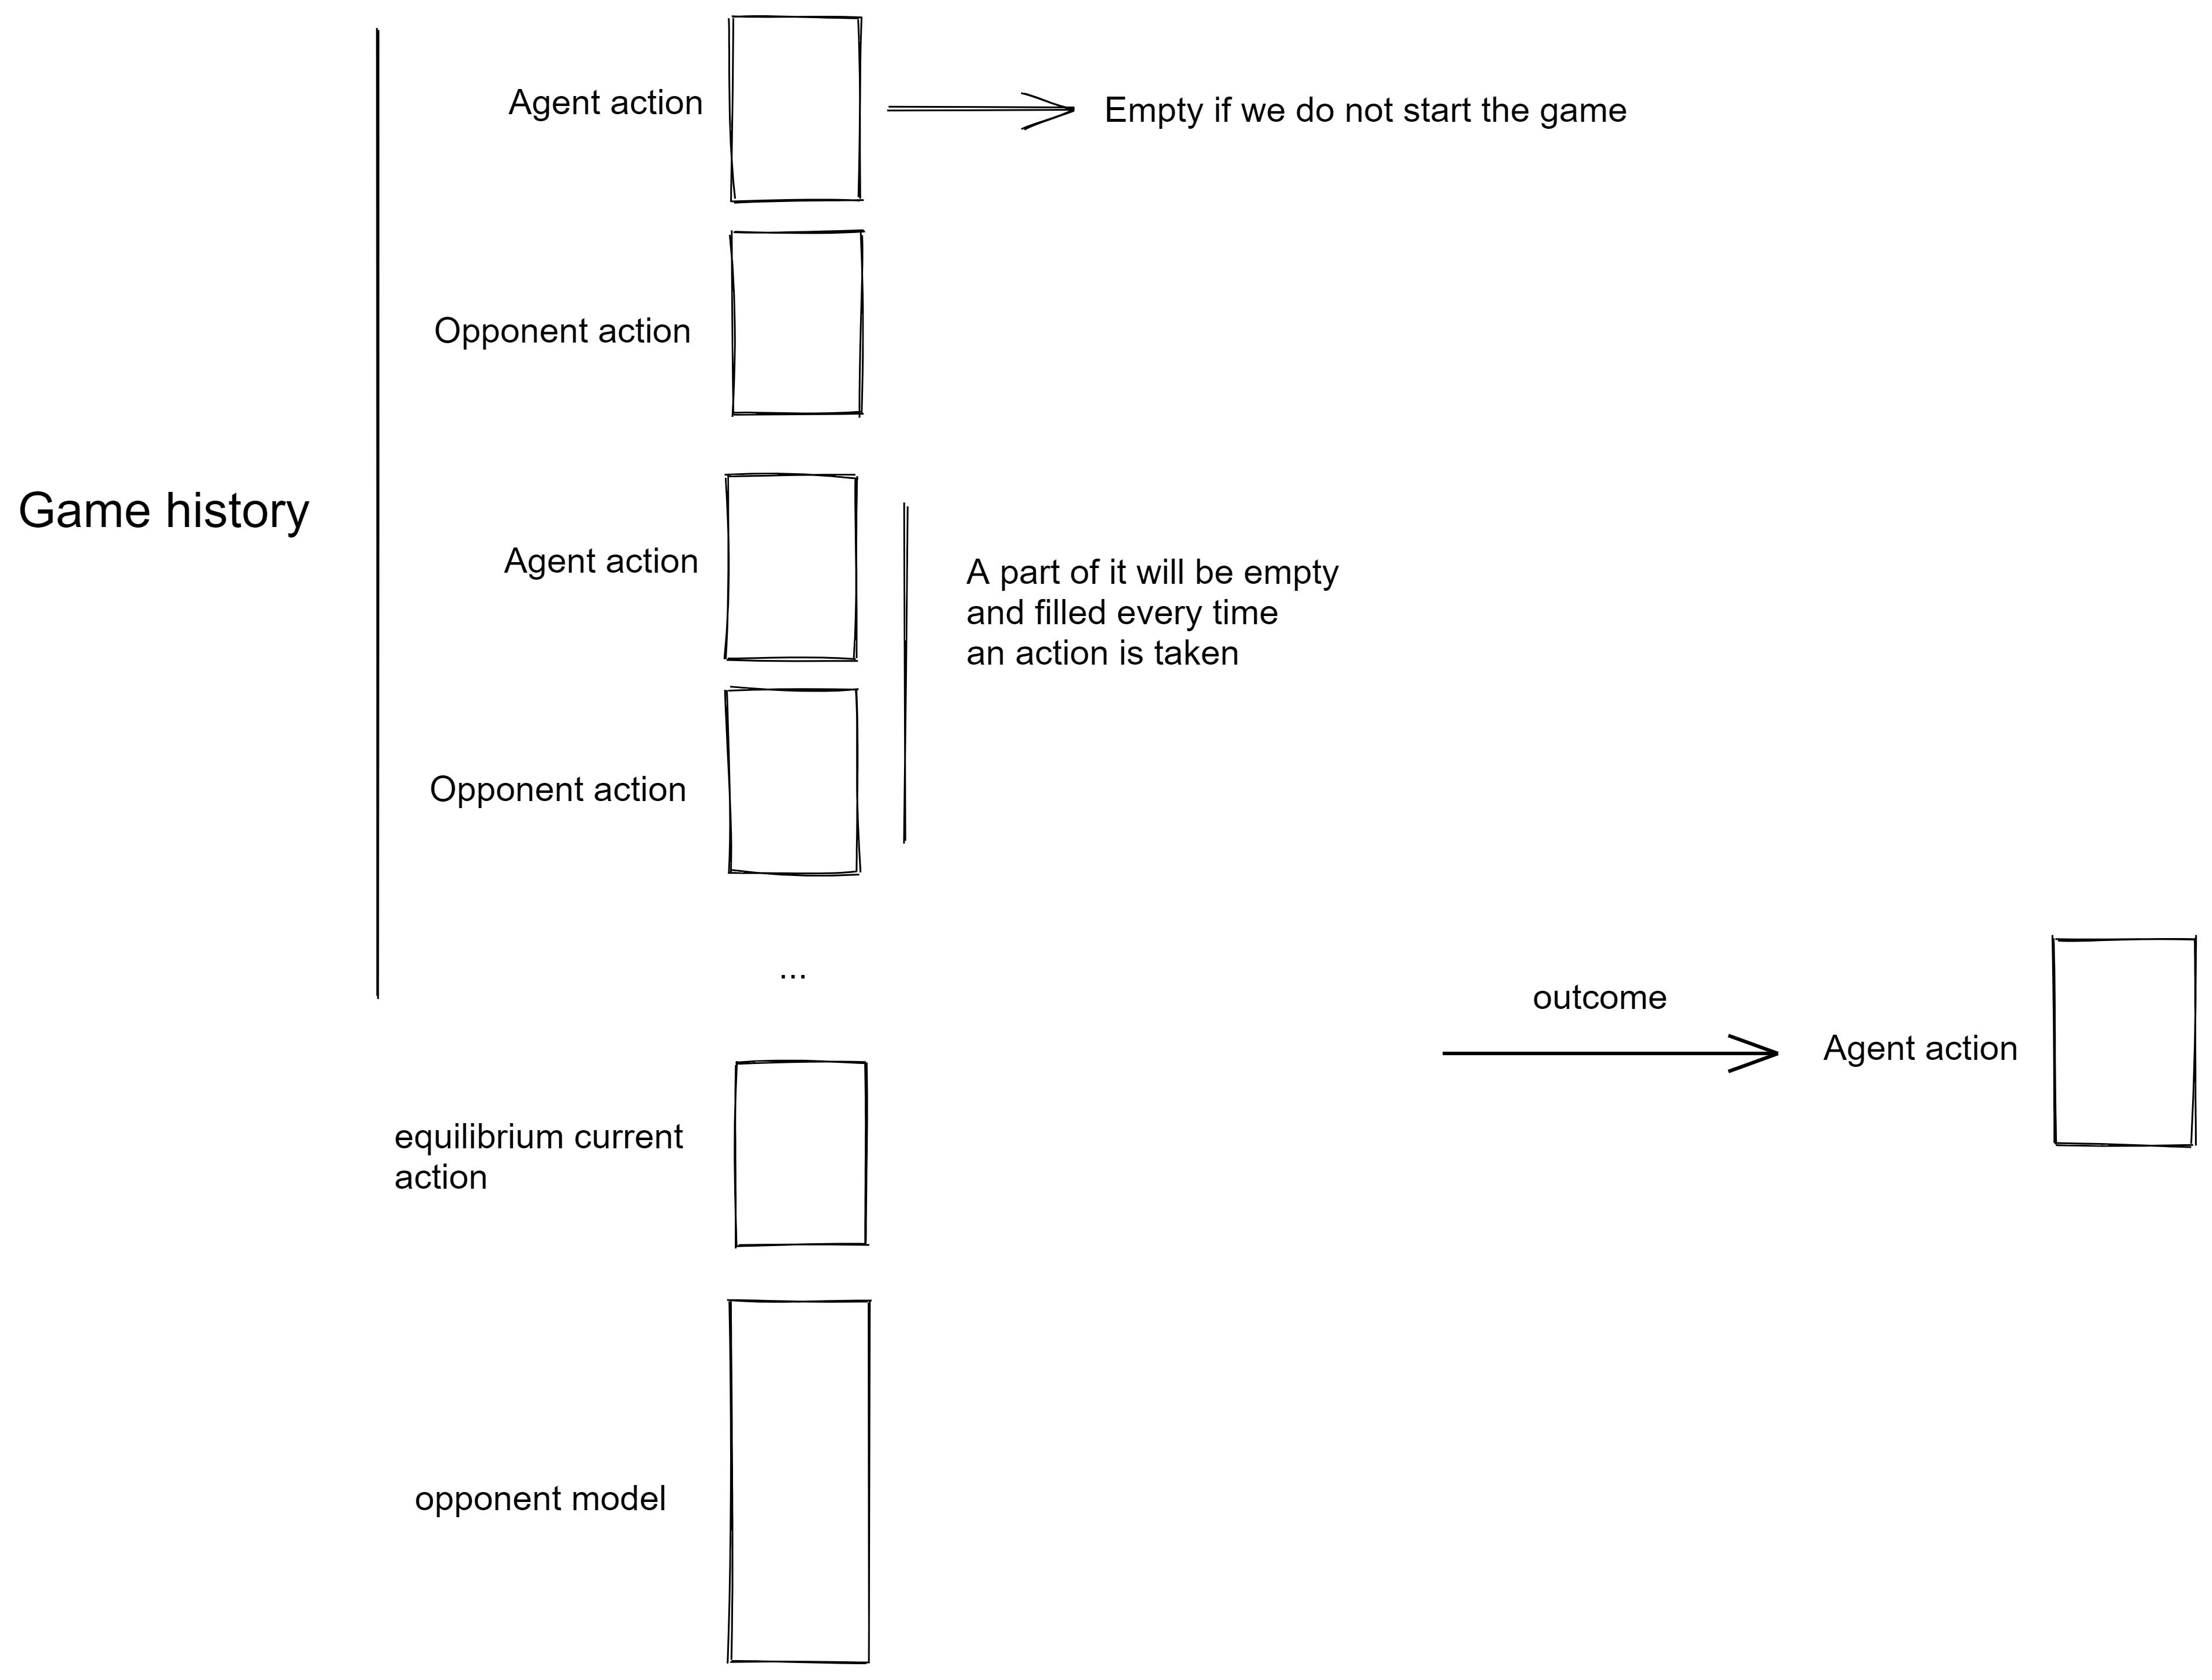
\includegraphics[width=1\textwidth]{Figures/decision-making-nn.png}
    \caption{Decision making NN}
    \label{fig:decision-making-nn}
\end{figure}

\section{Training Neural Networks}
The training of these neural networks is challenging and is the core difficulty of this project. Indeed we do not just expect our algorithm to be the best on the long term. We also expect it to be able to detect and exploit opponents.

\subsection{Attribution of reward}
We can not attribute or pre-compute the expected result given an input. Indeed the opponent modeling and decision making are too complex to calculate this. Instead, we attribute a reward given the actions taken by the agent.

The attribution of a reward is subtle and should be done carefully. We can not have a reward for every action the agent is making, it is not an instant reward.

For example, if the agent bet with bad cards maybe it is his strategy to exploit the opponent who is afraid when the agent bet. Given so we can not assign a negative reward to this action because the action takes part in a more advanced strategy. The reward needs to be given when the agent loses or wins something. In our case, if the agent ends up winning the game it will have a positive reward and a negative reward if it ends up losing the game.

It is a general idea of how attributing the reward, this can be tune given the learning algorithm used.

\subsection{Learning environment} \label{methodology:learning-environment}
The learning environment needs to make sure that the agent can learn how to exploit complex behavior. This is a difficult constraint because it means that the agent must play against multiple sub-optimal opponents.

This requires to have generated opponents created by the learning environment or/and have opponents with a fixed strategy defined before the learning starts. Having only opponents with a fixed strategy will cover only a few behaviors. Also, it makes complicated for this algorithm to be used in other imperfect game because it will require to find/create other opponents. So having only fixed strategies while learning should be avoided.

\subsection{Training algorithms}
We consider two kinds of algorithms that fit the training constraints. Competitive co-evolution and reinforcement learning.

\subsubsection{Competitive co-evolution} \label{methodology:competitive-co-evolution}
Competitive co-evolution (section: \ref{LR:competitive-co-evolution}) is the most promising kind of algorithm in its capacity of generating complex opponents and attributing a dynamic reward.

Competitive co-evolution makes multiples agents compete against each other. So it generates a set of sub-optimal opponents by design and makes it evolve into more complex agents over the training. Also, these agents start with simple behavior and the more the training continues more complex these agents became. It allows having incremental learning from simple to complex behavior.

Competitive co-evolution allows by design to have shared fitness. As said in section \ref{LR:competitive-co-evolution} it allows to promote diversity and encourage the development of promising behavior.

For evolving a NN with this algorithm, every weight needs to be encoded in a solution. Usually, EA has trouble scaling when the search space is too large. Neural networks tend to have a lot of weight, this can lead to performance issues if we are using EA to evolve it.

\subsubsection{Reinforcement Learning} \label{methodology:rl}
As said in section \ref{LR:reinforcement-learning}, reinforcement learning is made to work with rewards and have really good performance for evolving NN.

The main issue with this method is that it uses backpropagation to evolve the NN and it is hard to implement if multiple NN are involved. In our case, I think that backpropagation can be done even if we are using two NN. The reason is that a part of the decision-making input is the output of the opponent modeling NN, so we can theatrically propagate the error from one NN to the other. However, this would require extra research and work to implement it.

The second issue is that by design reinforcement learning does not work with multiple agents, in fact, it only evolves one NN. To meet our learning environment constraint (section: \ref{methodology:learning-environment}) we would need to manually find/create opponents with a fixed strategy. This is something we should avoid.

\subsection{Conclusion}
To conclude Competitive co-evolution perfectly fit the learning environment but may suffer from performance issue if the size of the NN is too important. On the other hand, reinforcement learning has really good performance for evolving NN but the solution is likely to be incomplete and suffer from a lack of diversity in the learning environment.

\section{Evaluation} \label{requirement:evaluation}
The evaluation is a crucial process for this research. It is the only way to demonstrate the capacity of neural network to model opponent behavior. Better the testing will be, the better these results will be generalized, without the need to run more experiments.

We will use poker to run our experiments. It is the most used game in imperfect game solving research as it includes complex behavior and strategy. The poker variant used will depend on the size of the game state we want to test.

Performances will be measured in milli-big blinds per hand (mbb/hand), the average number of big blinds win per 1000 hands. This is a common unit in poker research. Following this standard will allow these results to be comparable with other research papers.

\subsection{Exploitation testing} \label{requirement:evaluation:exploitation}
The exploitation testing will ensure that the algorithm successfully extracts simple opponent behavior. Even "stupid" opponents can be interesting to study because they can give metrics on how fast the algorithm exploits them.

Here is the list of the different algorithms:
\begin{itemize}
    \item Always fold
    \item Always rise
    \item Random: plays random moves
\end{itemize}

\subsection{Exploitability testing} \label{requirement:evaluation:exploitability}
Exploitability testing will provide information on how much the algorithm is exploitable.

It will play against an opponent following the equilibrium strategy. Given that, we will be able to see how reasonable our algorithm is and how well it managed to not fall into trying to exploit the equilibrium.

It will also be evaluated using the true best response with access to the private game state. In other words, at each step, the true best response will be computed with access to the card of every player. This is a non-realistic testing because it is cheating but it provides an interesting insight into how much the algorithm is exploitable.

We will also evaluate how far the algorithm is flexible and able to adapt if the opponent drastically switch his strategy. To do so we will have an opponent playing random for 100 games then playing the true best response for the remaining of the day.

\subsection{Advanced opponent testing} \label{requirement:evaluation:advanced}
In this testing category, we are trying to reproduce real-world poker examples. We will challenge our algorithm with different sub-optimal opponents.

We will use made up sub-optimal strategy by playing each action with a probability chosen uniformly randomly within 0.2 of the equilibrium probability. This type of sub-optimal opponent has been used in previous research in opponent modelling \citep{ganzfried2015safe}. It will be easier to compare the results.

We discard the usage of human testing for this research because it will require financial resources to have non-bias and conclusive results.

\chapter{Kuhn poker experiment} \label{kuhn-poker}

\lhead{Chapter 4. \emph{Kuhn poker experiment}}
In this chapter, we will present and explain the experiment on a simplified version of poker, the Kuhn poker.
First, we will describe how we setup the neural network and how we trained it. Then we will present the result and the different metrics on how well the neural network performed. Finally, we will analyze the result and try to generalize them to any imperfect game.

\section{Setup} \label{kuhnexperiment:setup}

\subsection{environment}
We created a Kuhn poker environment that gives us all the necessary data to correctly feed the neural network. We have defined 3 actions possible: check, bet and fold. We have decided to regroup raise and bet in the same action "bet" to reduce the complexity. If at any time the decision-making NN predicts an incorrect action, the default action "bet" or "check" would be done.

\subsection{NN}
We decided to first use a simple RNN for the opponent modeling, you can find more information about the specific input of this NN in section \ref{methodology:opponent-modelling}, see figure \ref{fig:opponent-modelling-nn-rnn}. We used the decision making NN describe in section \ref{methodology:descision-making}, figure \ref{fig:decision-making-nn}.

Different layers size has been tested, from 10 to 20 for the hidden layer size of the descision making NN and from 5 to 20 for the opponent modelling NN. We also tried to add an other hidden layer for both NN. activation function, and opponent model size has been tested. We did not notice any improvement while increasing the layer size above 10 for both NN.

Different activation function has been tried, linear, sigmoid and relu. The result between the sigmoid and the linear function are pretty similar. However the relu had bad performance compared to the linear.

Different opponent model size has been tested, from 5 to 20. While analyzing the neural networks we have seen that the decision making NN uses at most 5 input, the others were not impacting the decision. However it is worth to notice that due to the way our training is done, it makes sense to use a larger opponent model size because we can not except all the opponent model output to be meaningful.

Only the most successful architecture will be presented, their results will be detailed in the section \ref{kuhnexperiment:result}. The descriptions of their NN layers are detailed in table \ref{tab:nn-layer-kuhn}. The size of the input layer is defined by the environment and the opponent model size. It has been detailed in the section \ref{methodology:NN}. 

\begin{table}[ht]
\centering
\begin{tabular}{ |c|c|c| }
 \hline
 NN name & opponent-modelling NN  & descision-making NN \\ 
 \hline
 input layer & x & x \\ 
 \hline
 hidden layer & 10 & 10 \\
 activation & linear & linear \\
 \hline
 output layer & opponent model size & 3 (check, bet, fold) \\
 activation & sigmoid & softmax \\
 \hline
\end{tabular}
\caption{NN layer (kuhn poker)}
\label{tab:nn-layer-kuhn}
\end{table}

\subsection{Training}
To train the NN we have used competitive co-evolution, general information about it can be found in section \ref{methodology:competitive-co-evolution}.

We have used these strategy in the teaching set:

\begin{itemize}
    \item \textbf{Equilibrium}: playing the equilibrium strategy
    \item \textbf{Random}: playing a random action in the set of the available ones
    \item \textbf{Always bet}
    \item \textbf{Always fold}
    \item \textbf{Close Equilibrium}: playing a strategy close to the equilibrium. It select each action with a probability chosen uniformly randomly within 0.2 of the equilibrium probability. It aims to produce realistic sub-optimal opponent.
\end{itemize}

We have by default added 3 different \textit{Close Equilibrium} strategies to the teaching set. We have not used a system to dynamically add training agents to the teaching set. We are making each agent playing against each other and using a shared fitness to promote diversity (ref: \ref{LR:competitive-co-evolution}). To make the result of the games not based on cards luck, we are first making the two agents play a set of rounds. Then, we erase their memory and make them play with the opposite cards. A temporary reward is attributed, the agent winning 1, the one losing -1, then the final reward is attributed after the shared fitness calculation.

The EA has been used with these parameters. These parameters have been decided after multiple iterations, those seem to have good training performance in this context. For reference, we have put in italic the range of the values that we looked at.
\begin{itemize}
    \item population size: 20 ; \textit{10 to 25}
    \item individual kept each iteration: 5 ; \textit{2 to 5}
    \item mutation rate: 0.1 ; \textit{0.1 to 0.2}
    \item iteration: 100 ; \textit{10 to 100}
    \item number of rounds (games): 25 ; \textit{5 to 25}
\end{itemize}

You can find pseudo-code for the EA in the appendices \ref{lst:ea-training}.

\section{Result} \label{kuhnexperiment:result}
To evaluate the NN we apply the evaluation method detailed in the section \ref{requirement:evaluation}.

In this section, results of multiple NN models will be presented, the NN and EA parameters are by default the one described in the previous section \ref{kuhnexperiment:setup}.

\begin{itemize}
    \item \textbf{Classic}: No parameters changes.
    \item \textbf{More Games}: Playing 50 games per iteration (instead of 25). Only 10 individuals and 3 are kept at each iteration.
    \item \textbf{Bigger Model Size}: The opponent model size is 10 (instead of 5)
    \item \textbf{Larger Teaching Set}: Having 6 \textit{Close Equilibrium} agents in the teaching set
\end{itemize}

Due to the limited resources, the models are from a single run of the EA. For the record, one run takes approximately 2h, performances are discussed in section TODO-SECTION-SCALE-UP.

\subsection{Win rate}

In this section we will present the win rate of the different tested models against multiple strategies, the choices of these strategies are detailed in the section \ref{requirement:evaluation}.  We made the agents played together 500 games, erased their memory then played another 500 games with the opposite cards. You can find the results in the table \ref{tab:reward-kuhn}.

It is worth mentioning that the \textit{Close Equilibrium} strategy during the evaluation is not one of the training set.

\begin{table}[h]
\resizebox{\textwidth}{!}{
\begin{tabular}{ |c|c|c|c|c|c|c|c| }
 \hline
 Opponent Model & E & Close E & Random & Always Bet & Always Fold & TBR & Random then TBR \\ 
 \hline
 Classic & 0.001 & 0.053 & 0.202 & 0.293 & 0 & -0.182 & -0.139 \\
 \hline
 More Games & 0.006 & 0.001 & 0.312 & 0.200 & 0.646 & -0.175 & -0.116 \\ 
 \hline
 Bigger Model Size & -0.02 & 0.027 & 0.309 & 0.180 & 0.106 & -0.087 & -0.065 \\
 \hline
 Larger Teaching Set & 0.001 & 0.054 & 0.196 & 0.350 & 0 & -0.172 & -0.120 \\
 \hline
 Equilibrium & 0 & 0.007 & 0.150 & 0.104 & 0.238 & -0.125 & -0.118 \\
 \hline
\end{tabular}
}
\caption{Win rate in mbb/hand of the opponent model against evaluation opponent for the kuhn poker (Equilibrium has been shortened to E and true best response to TBR)}
\label{tab:reward-kuhn}
\end{table}
\subsubsection{Sub-optimal opponent exploitation}

We can see that the model \textit{Classic} have really good performance against \textit{Close Equilibrium} (0.054) compared to the equilibrium (0.007). It demonstrates the capacity of the NN model to exploit sub-optimal opponent.

In the study \citep{ganzfried2015safe}, they have an agent playing the best response according to the opponent model that they use for reference to demonstrate how unsafe it is. This algorithm have similar result as \textbf{Classic} regarding the \textit{Close Equilibrium} (called sophisticated static in this study). However, the main difference is that the model \textit{Classic} is less exploitable. Indeed comparing the difference between equilibrium and the algorithm for the random then TBR (called dynamic in the other study). It gives us 0.021 for \textit{Classic} and 0.085 for the best response in the study. To sum up, using NN we are capable of achieving as good results as algorithms fully committed to opponent exploitation while being less exploitable.

\subsubsection{Impact of training}

We can notice that model \textit{Classic} and \textit{Larger Teaching Set} perform poorly against always fold, an opponent that is supposed to be easily exploitable. We can assume it is linked to the way NN are trained. In competitive EA with shared fitness, it is likely that a strategy exploiting a stronger opponent (always bet) will have a better fitness compared to exploiting a simple opponent (always fold). Polishing the EA training would likely improve and stabilize the results over multiple runs.

In addition EA are known to be stochastic, meaning that the results are hard to be predictable. That is because of the random elements such as the initialisation, selection and mutation. To have a good and predictable result, you are likely going to need to run multiple times the process and select the best of them.

\subsubsection{Exploitability}

The true best response help understands how much an algorithm is exploitable, it has access to every player's cards and plays the best response every time. It is not an absolute metric but highlight if an algorithm is likely to be exploitable.

An interesting thing about the \textit{Bigger Model Size} model result is that it performs better than the equilibrium against the \textit{TBR} and \textbf{Random then TBR}. Both of these strategies are "cheating" by having access to the opponent private information to produce the true best response. We can assume that the NN is noticing that the opponent is particularly good and decide to play super safe minimizing the loss. It demonstrates that using NN to model the opponent is not easily exploitable. Most important, it demonstrates that it can reduce the exploitability if the opponent is aware of a part of your private information.

In real-life use cases, it is frequent that some of your private information is known by the opponent. For example, if you are negotiating a deal, the person may know the budget of your company while you think it is private information.

\subsection{Reward over time}

In this section, we will present the interesting plots of the reward over time for different models.

The different plots showcase in this section are based on 1000 played games. It is worth to note that the EA training has been run having only 25 games played between each agent. Using a different scale (from 25 to 1000) demonstrate how the NN model handle keeping an opponent model through more game than usual.

\begin{figure}[ht]
    \centering
    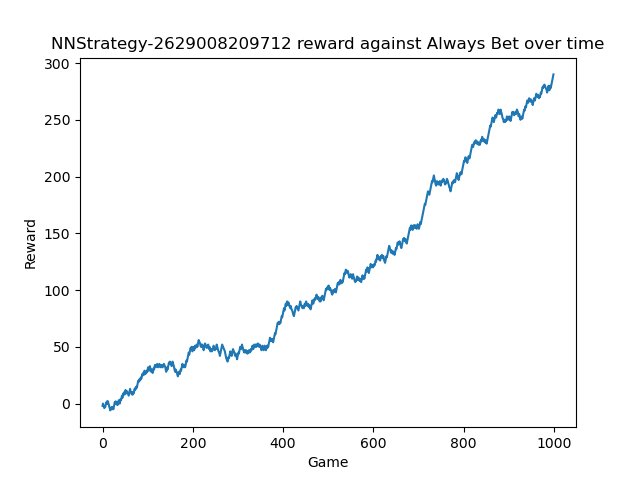
\includegraphics[width=0.7\textwidth]{Figures/out-plots/kuhn/larger-teaching-set/reward-against-Always Bet.png}
    \caption{Model Larger Teaching Set, reward against Always Bet over time}
    \label{fig:kuhn:larger-teaching-set-always-bet}
\end{figure}

In figure \ref{fig:kuhn:larger-teaching-set-always-bet}, you can see that at the very beginning, the reward is neither increasing nor decreasing. Then after some games, we can assume that the NN draws a model of the opponent, and start to exploit it by having a relatively stable increase of the reward.

\begin{figure}[ht]
    \centering
    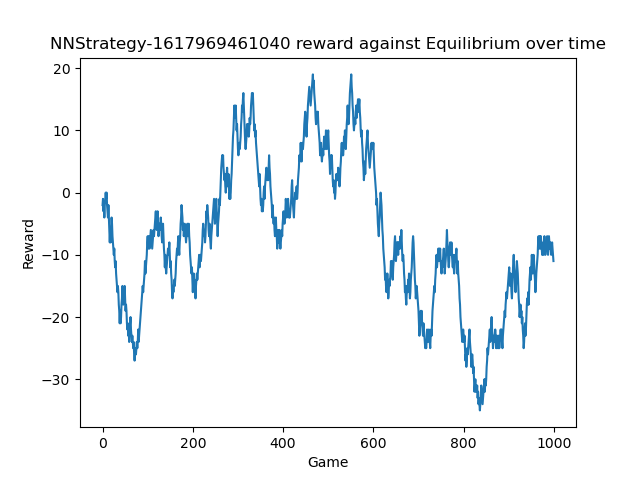
\includegraphics[width=0.7\textwidth]{Figures/out-plots/kuhn/more-games/reward-against-Equilibrium.png}
    \caption{Model More Games, reward against Equilibrium over time}
    \label{fig:kuhn:more-games-equilibrium}
\end{figure}

In figure \ref{fig:kuhn:more-games-equilibrium}, you can see that there is not a straight tendency of increasing or decreasing. It's what you expect from a game against two opponents without net exploitation. It demonstrates the ability of the model to not fall into a wrong interpretation or at least recover/correct the opponent model.

\subsection{Input impact on the NN} \label{kuhnexperiment:result:input-impact}

We have measured the impact of each input to every output of the neural network to determine how much the input is taken into consideration in the decision. To do that we used SHAP \citep{shap}, a game-theoretic approach to explain the output of any machine learning model. On the plots, inputs are ordered by impact. Each blue dot represents the impact (positive or negative) of one input for one activation.

\begin{figure}[ht]
    \centering
    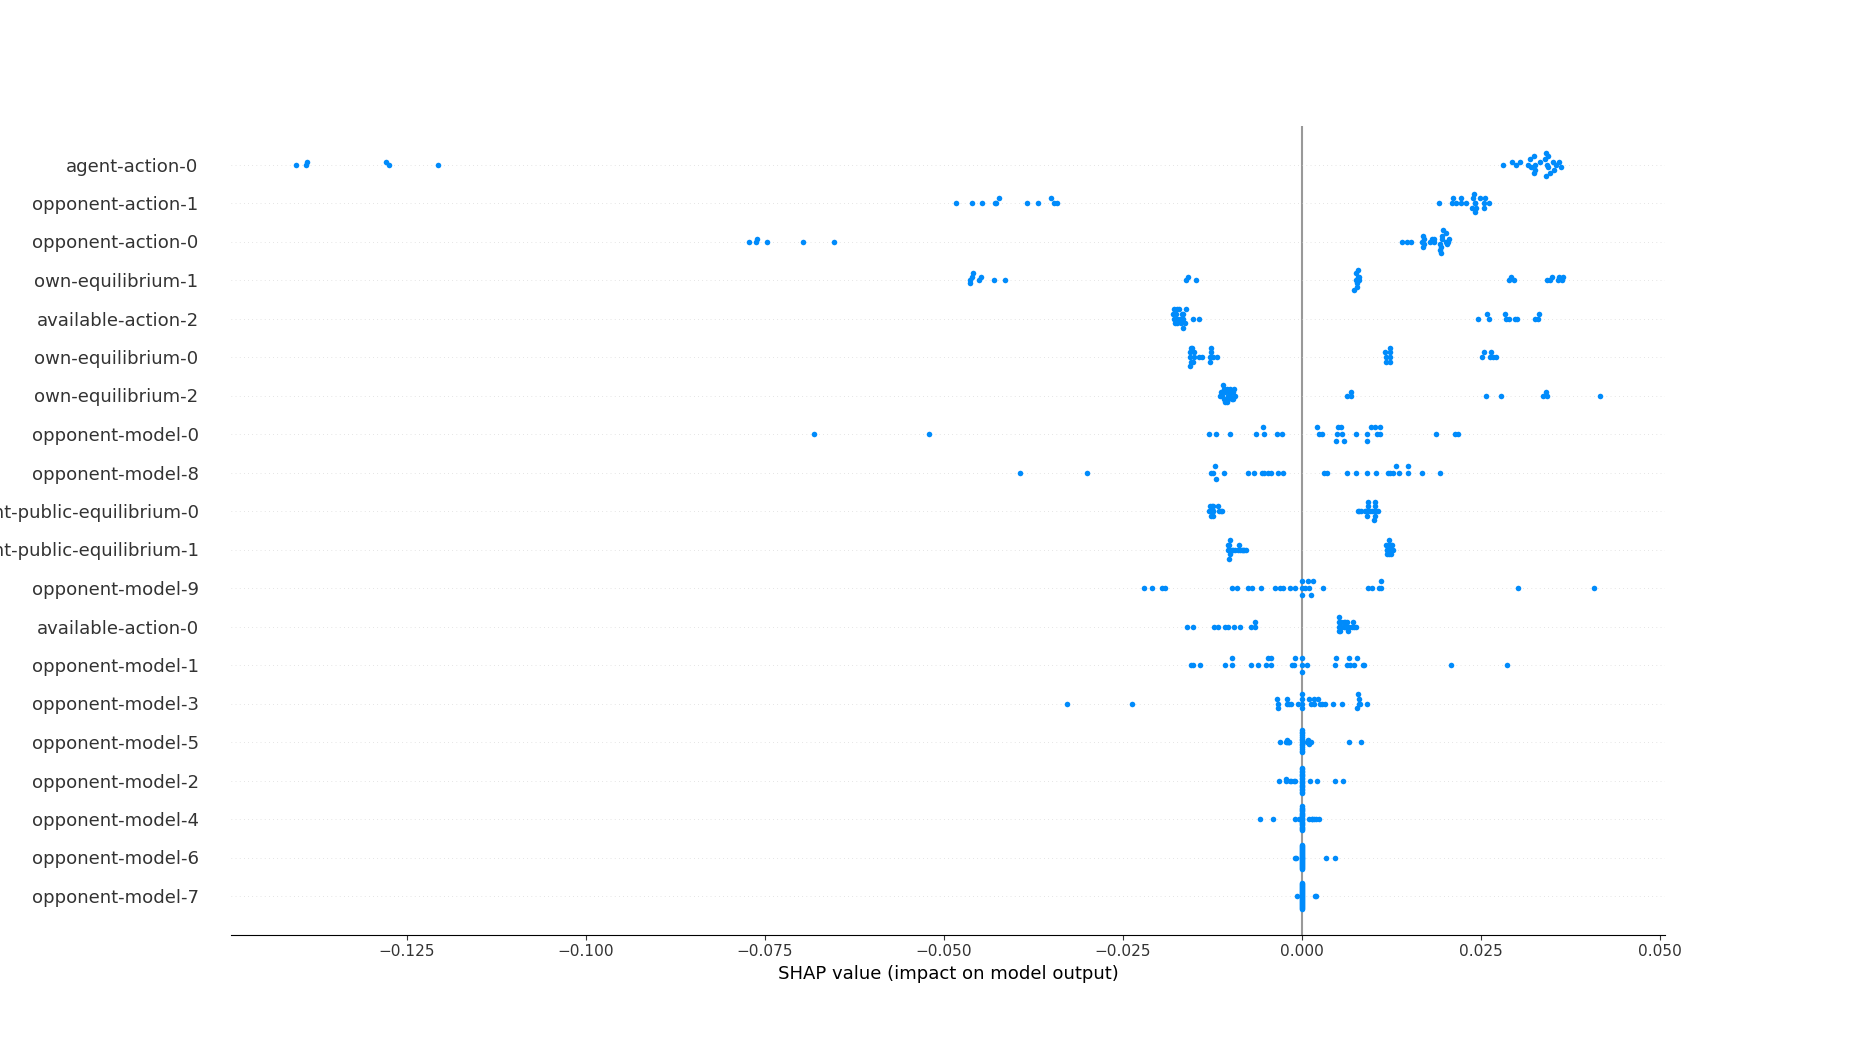
\includegraphics[width=1\textwidth]{Figures/out-plots/kuhn/bigger-model/action-check-input-impact.png}
    \caption{Bigger Model Size, input impact for the check action}
    \label{fig:kuhn:bigger-model-impact-check}
\end{figure}

\begin{figure}[ht]
    \centering
    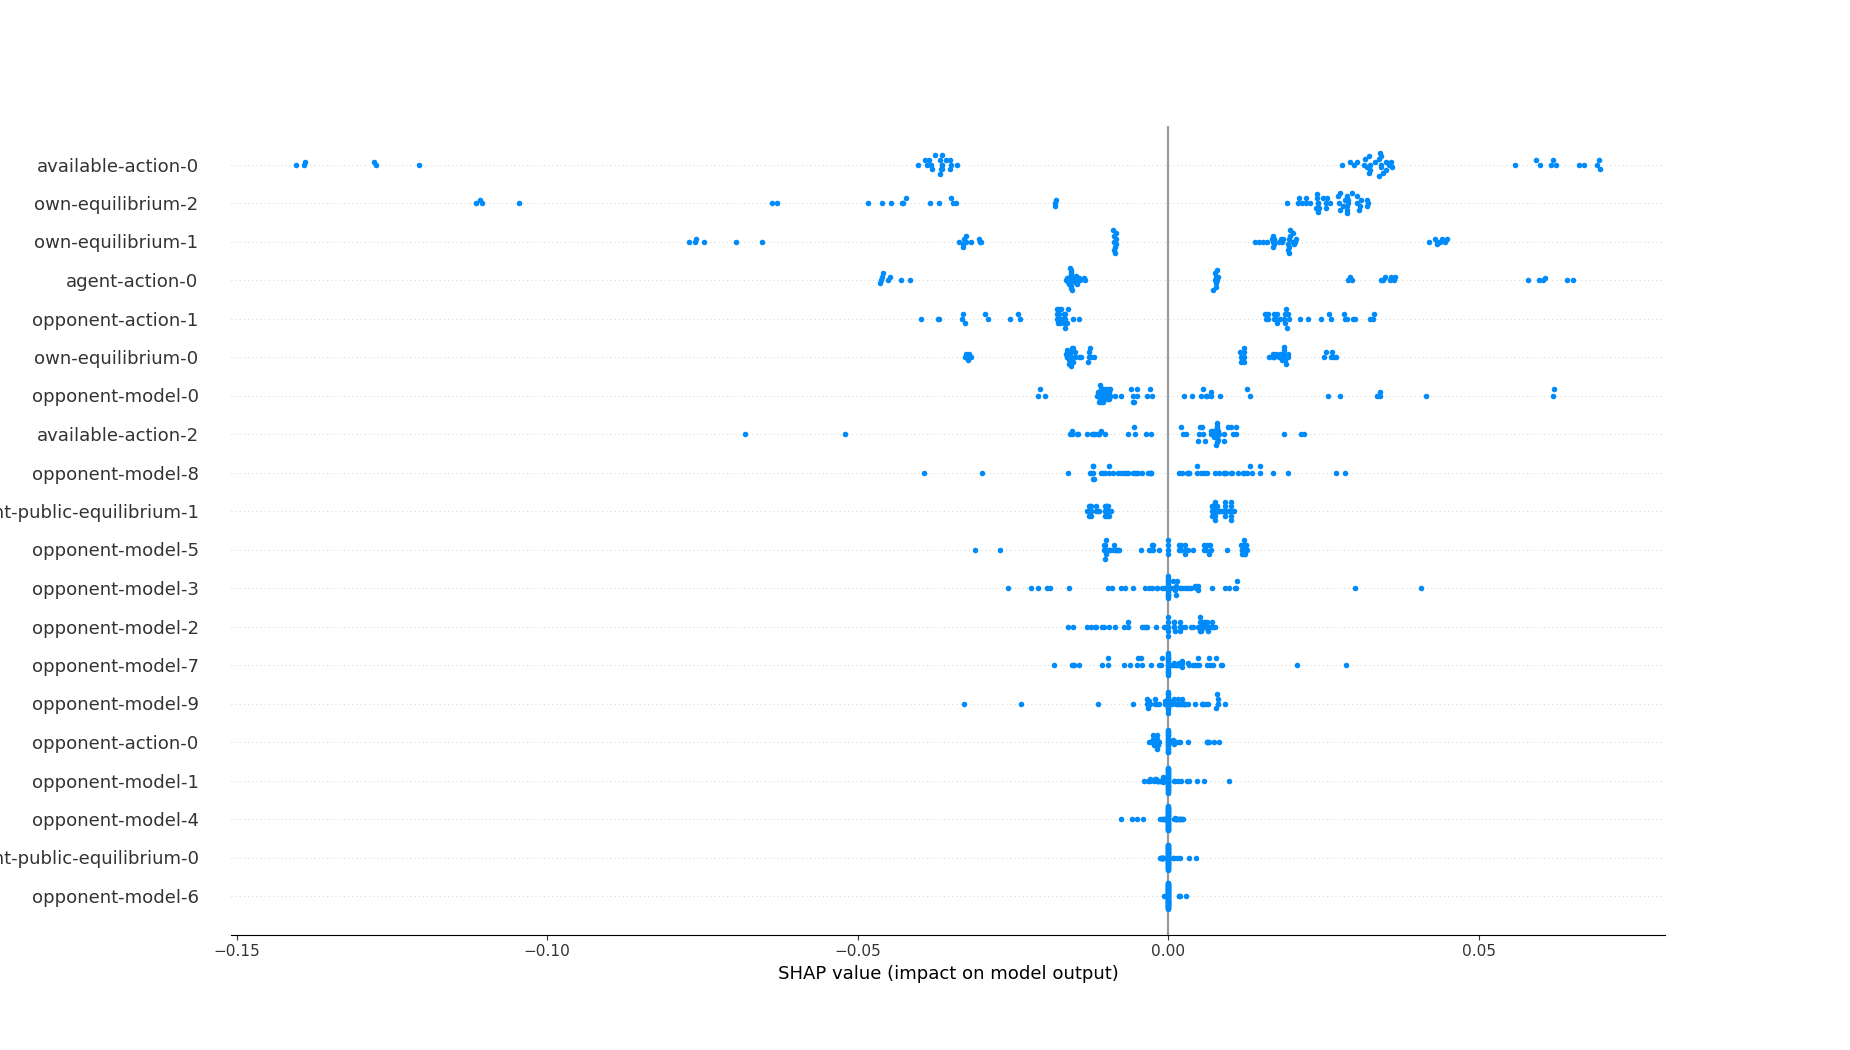
\includegraphics[width=1\textwidth]{Figures/out-plots/kuhn/bigger-model/action-bet-input-impact.png}
    \caption{Bigger Model Size, input impact for the bet action}
    \label{fig:kuhn:bigger-model-impact-bet}
\end{figure}

For the model \textit{Bigger Model Size}, we can see that on the opponent-model-0 input is part of the most impacting input for the bet and check action, figure \ref{fig:kuhn:bigger-model-impact-check} and \ref{fig:kuhn:bigger-model-impact-bet}. It demonstrates that the NN relies on the opponent model to take its decision.

\begin{figure}[ht]
    \centering
    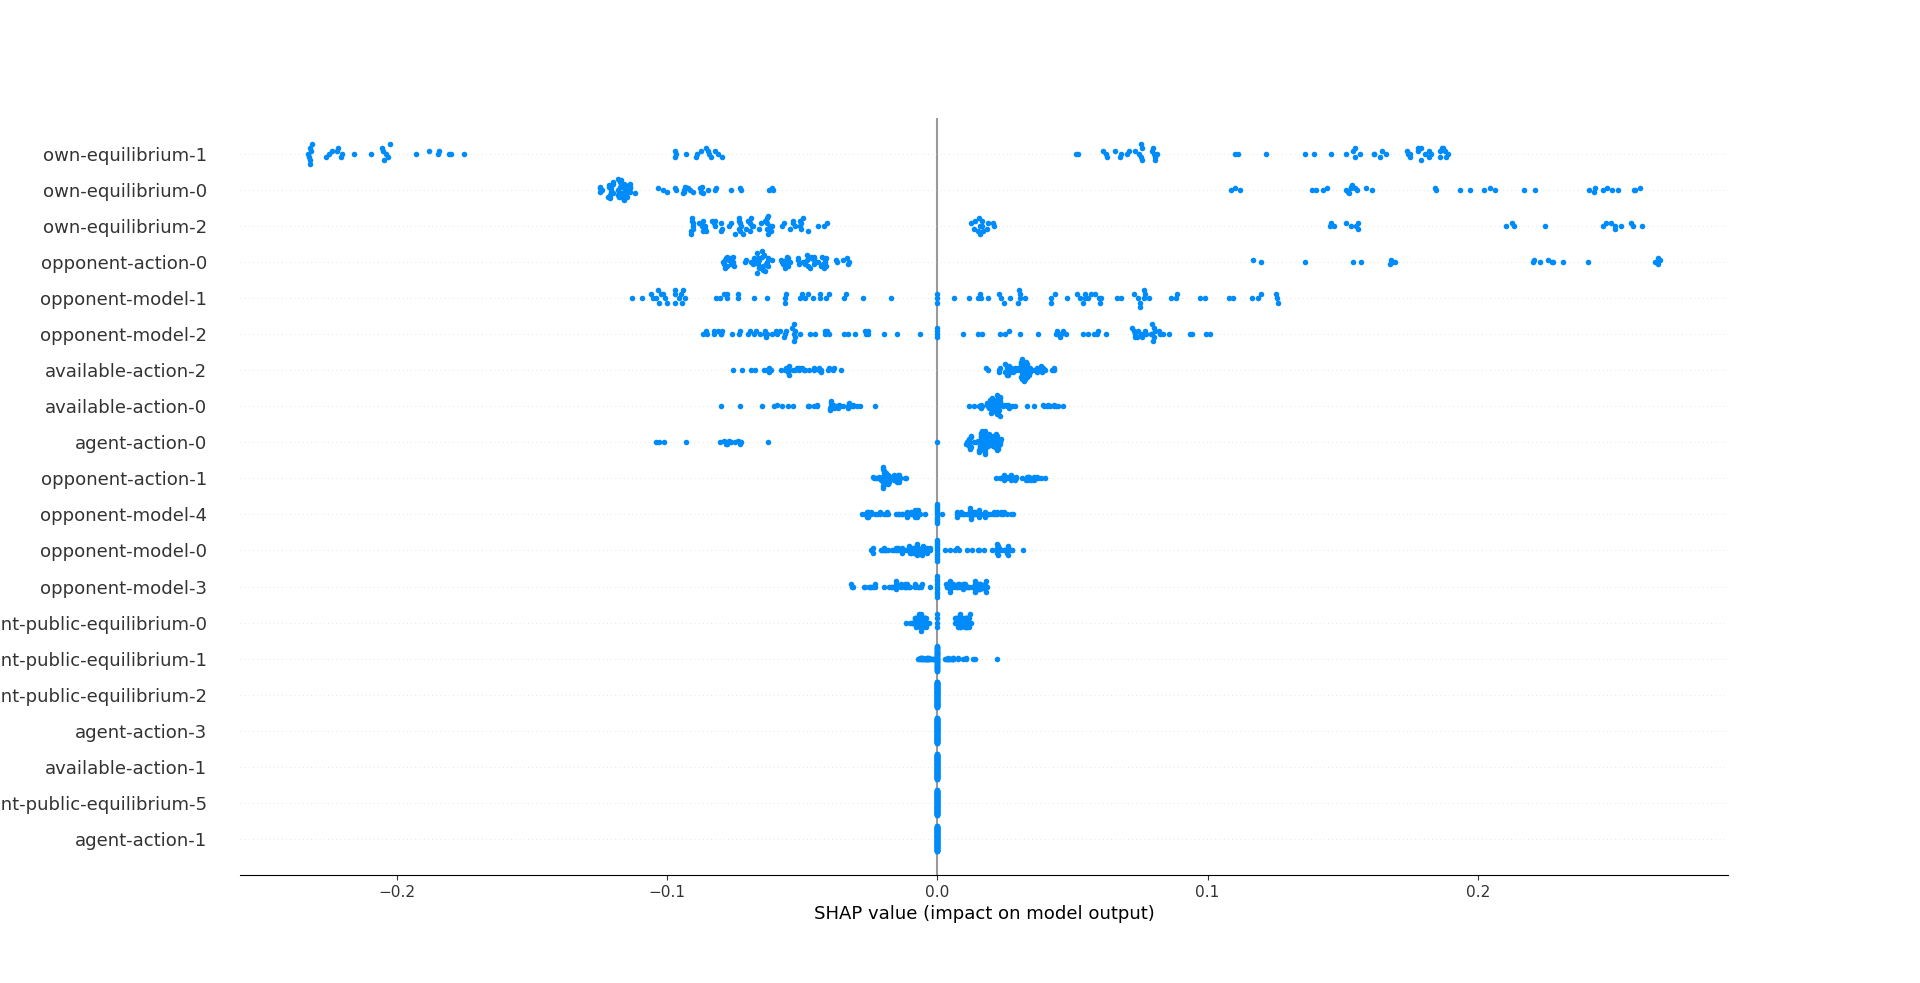
\includegraphics[width=1\textwidth]{Figures/out-plots/kuhn/A/action-fold-input-impact.png}
    \caption{Bigger Model Size, input impact for opponent-model-0}
    \label{fig:kuhn:bigger-model-impact-opponent-model-0}
\end{figure}

For the model \textit{Bigger Model Size} we can also analyze how the "opponent-model-0" is made by analyzing the opponent model NN, figure \ref{fig:kuhn:bigger-model-impact-opponent-model-0}. We can see that the most used inputs are the game outcome, the first opponent action, and the first agent action. Interpreting the purpose of this opponent model output is hazardous because NN are complex. For example, a possible analysis is that this part of the opponent model aims to define if the opponent is often winning when he is betting.

\section{Analysis}

\subsection{Approximation or incorrect Equilibrium}

During the development, I had a bug that allowed cards to be draw multiple times. It was possible to have the player one king and the second with another king (which is not possible in the Kuhn poker). So it makes the equilibrium incorrect. Even if the equilibrium was incorrect it managed to overcome this and exploit the different strategies. This means that using NN to exploit opponents in imperfect games using this NN architecture can manage and overcome incorrect or approximated equilibrium.

It is worth mentioning that the performances are likely to be degraded because the NN will need to learn the game. Indeed it will likely rely on the game history such as the previous action instead of relying on the equilibrium.

Obviously, this bug has been fixed and the presented result in the previous section are with the correct version.

\section{Conclusion}

With this Kuhn poker experiment, we can draw some general conclusions about opponent exploitation with neural networks in imperfect games.

We have demonstrated the capacity of a NN to model and exploit an opponent.

We have seen that it is way less exploitable than other existing algorithms used to model the opponent. Some models were having really good exploitability results, even better than equilibrium. Demonstrating that they were able to reduce their exploitability if the opponent knew some private information.

We have also highlighted the importance of the training phase and its impact on the quality of the model.

To conclude using NN to model opponents achieves as good results as existing algorithms while being way less exploitable than them.

% Chapter Template

\chapter{Scale up, limit texas holdem poker experiment} % Main chapter title

\label{scale-up}

\lhead{Chapter 5. \emph{Scale up, limit texas holdem experiment}} % Change X to a consecutive number; this is for the header on each page - perhaps a shortened title

\section{Introduction}
In this chapter, we will study how well our algorithm is scaling up on more complex games. To do this we are going to adapt our algorithm to make it works with the limit texas holdem poker variant. This game has an info set size of \(10^{14}\) and 5 available actions.

\section{Equilibrium approximation}
One of the most complex tasks is to approximate the equilibrium. As discussed previously, a lot of algorithm aims to find a good approximation of the equilibrium and it is an active field of research (ref: \ref{LR:section:imperfect-game-solving}). There is a lot of complex algorithm with specific optimization. We decided to implement an algorithm called CFR (Counterfactual Regret Minimization) \citep{CFRIntoHeller2013introduction}.

Approximating the equilibrium takes a relatively high amount of time, to increase the performances we implemented it in C++ and bound it to our python program.

\subsection{CFR}
CFR algorithm is a machine learning decision tree algorithm. For each iteration, it explores the whole tree with a given starting state. Once it reaches the terminated nodes it can assign a regret to it given the result of the game. This regret is then back-propagated taking into account the probability to reach this node. The probability to reach this node is calculated by creating strategies for each state transition. The goal of these strategies is to find the optimal probability for the player playing. These strategies are updated at every iteration given the regret of the leading nodes. Because this algorithm is applied in a two-player game, it requires paying extra attention to inverse the regret at every step so that each player will try to minimize their regret. You can find the pseudo-code of this CFR in \ref{lst:cfr}.

\section{Experiment}
\subsection{Setup} \label{scale-up:experiment:setup}
We used the same setup as for the kuhn poker experiment (ref: \ref{kuhnexperiment:setup}). We tried to run it with the following hyper-parameters. They were choose to balance the time a game takes by reducing the overall number of games in one iteration.
\begin{itemize}
    \item population size 10
    \item individual kept each iteration 3
    \item mutation rate 0.2
    \item number of games 10
    \item iteration 200
\end{itemize}

Running one iteration takes 2h30. Due to a lack of resources, I was not able to properly run all the iterations. However, we can still think about how realistic it is to run this algorithm.

\subsection{Number of trainable parameters}
The number of trainable parameters is simply the number of weights and bias in the neural network. Using the same NN layers like the one for the kuhn experiment \ref{kuhnexperiment:setup}, we were able to extract these numbers, you can find it in table \ref{tab:trainable-parameters}.

\begin{table}[h]
\begin{center}
\begin{tabular}{ |c|c| } 
 \hline
 Game & Number of trainable parameters \\ 
 \hline
 Kuhn poker & 754 \\ 
 \hline
 Limit texas holdem poker & 6000 \\ 
 \hline
\end{tabular}
\end{center}
\caption{Number of trainable parameters}
\label{tab:trainable-parameters}
\end{table}

We can notice that there are only 8 times more trainable parameters (\(6000/754 \approx 8\)). We can assume that the training will need 8 times more iterations, so we can approximate the training time: \(2h30 * 8 * 100 \approx 83 days\). However there is a huge margin to reduce this training time, it will be discussed in the next section \ref{scale-up:optimisation}.

\section{Optimisation} \label{scale-up:optimisation}
The \(83days\) of training were calculated given the specs of my computer (i7-9750H CPU @ 2.60GHz, rtx2060 GPU and 16GB of RAM).

\subsection{Multi-threading} 
The first way to drastically improve the performance would be by multi-threading all the games. Indeed almost all the training time is spent making agents playing against each other. Given this, the training time could theoretically be lowered to at least less than 30s per iteration in an optimum setup where each game has a dedicated thread. Even in a non-optimum setup, each thread reduces the training time.

\subsection{Equilibrium}
Another way to improve the algorithm performance on this poker version would be to optimize the time to compute the equilibrium approximation. Indeed, in this version, at least 80\% of the game time is spent computing the equilibrium. There is a famous algorithm called MCCFR (Monte Carlo Counterfactual Regret Minimization), studies have shown that its performance is at least 10 times better than the classic CFR \citep{MCCFRlanctot2009monte}, \citep{MCCFRlanctot2009monte}. Just with this update, this could theoretically bring the training time to \(\approx17days\) taking my computer for reference.

\section{Conclusion}
Scaling up the algorithm is doable, the number of trainable parameters seems to reasonably increase allowing complex games to be trainable. The scalability of the algorithm heavily relies on how fast it is possible to approximate the equilibrium. The more difficult the game will be, the more time it would require to compute the equilibrium and so slow down the training. By multi-threading the algorithm, with enough hardware resources, it is possible to train this algorithm on complex imperfect games in a reasonable amount of time.

%----------------------------------------------------------------------------------------
%	THESIS CONTENT - APPENDICES
%----------------------------------------------------------------------------------------

\addtocontents{toc}{\vspace{2em}} % Add a gap in the Contents, for aesthetics

\appendix % Cue to tell LaTeX that the following 'chapters' are Appendices

% Include the appendices of the thesis as separate files from the Appendices folder
% Uncomment the lines as you write the Appendices

% Appendix A

\chapter{EA training algorithm} % Main appendix title

\label{AppendixA} % For referencing this appendix elsewhere, use \ref{AppendixA}

\lhead{Appendix A. \emph{EA training algorithm }} % This is for the header on each page - perhaps a shortened title

\begin{lstlisting}[caption={EA training algorithm}, label={lst:ea-training},]
% data structure
Struct Individual {
    won_against = []
    lost_against = []
    fitness = 0
}

% The TeachingIndividual is only here for indication,
% you can have a different set of metadata
Struct TeachingIndividual extends Individual {
    strategy_name: string
}

Struct LearningIndividual extends Individual {
    values: array representing the training parameters
}

% hyperparameters
iterations = 100
mutation_rate = 0.1
trainable_params = 10
nb_population = 10
new_member_per_population = 7
individual_kept_nb = nb_population - new_member_per_population

% initialization
training_individuals = []
FOR _ in nb_population:
    training_individuals.append(LearningIndividual(
        values: random number array from -1 to 1 of size trainable_params,
    ))
teaching_individuals = [
    TeachingIndividual(strategy_name: "equilibrium")
    TeachingIndividual(strategy_name: "random")
    TeachingIndividual(strategy_name: "bet")
    TeachingIndividual(strategy_name: "fold")
    TeachingIndividual(strategy_name: "close_equilibrium")
]

% run
FOR _ in iterations:
    population = training_individuals + teaching_individuals

    % make them play against eachother
    FOR i = 0; i to population.size():
        FOR j = i + 1; j to population.size():
            a, b = population[i], population[j]
            result = evaluate(a, b)
            IF result == WIN:
                a.won_against.append(b)
                b.lost_against.append(a)
            ELSE IF result == LOST:
                b.won_against.append(a)
                a.lost_against.append(b)

    % assign fitness
    FOR individual in population.size():
        individual.fitness = 0
        FOR looser_individual in individual.lost_against:
            individual.fitness += 1 / looser_individual.lost_against.size()

    % generate new population
    selected_individuals = randomly select new_member_per_population
                             of training_individuals proportionaly to their fitness
    FOR new_individual in selected_individuals:
        new_individual.values = randomly change the values from -1 to 1
                                  with a probability of mutation_rate

    % process selection and assign a new population
    individual_kept = select individual_kept_nb best training_individuals
                        based on their fitness
    training_individuals = selected_individuals + individual_kept
\end{lstlisting}

% Appendix A

\chapter{CFR pseudo-code} % Main appendix title

\label{AppendixCFR} % For referencing this appendix elsewhere, use \ref{AppendixA}

\lhead{Appendix B. \emph{CFR pseudo-code}} % This is for the header on each page - perhaps a shortened title

\begin{lstlisting}[caption={CFR pseudo-code}, label={lst:cfr}]
Class PokerEnv {...}
% A class representing the poker env, it's implementation
% will not be shown in this pseudo-code

Struct StategyInfo {
    float value;
    string action;
}

Struct NodeInfo {
    % you should store an hash key of this env intead of
    % the full PokerEnv, we are doing this for readability
    PokerEnv env
    float regret
    Map<PokerEnv, strategys> strategys
}

nodes = {}

void runOnce(env, proba):
    currentNode = nodes[env]

    if (env.isOver()):
        currentNode.regret = env.reward * proba
        return

    actions = env.getAvailableActions()
    leadingNodes = {}
    total = 0

    % explore and compute values of the leading nodes
    FOR action in actions:
        copy = env.copy()
        copy.play(action)
        if (!currentNode.strategys[copy]):
            currentNode.strategys[copy] = {
                value: 1 / actions.size
                action: action
            }
        runOnce(copy, currentNode.strategys[copy].value * proba)
        leadingNodes.append(nodes[copy])

    sumNegativeRegret = 0
    sumPositiveRegret = 0
    for FOR node in leadingNodes:
        regret = -node.regret
        if (regret > 0):
            sumPositiveRegret += regret;
        else:
            sumNegativeRegret += regret;

    % update strategies
    FOR node IN leadingNodes:
        regret = -node.regret
        if (sumPositiveRegret > 0):
            currentNode.strategys[node.env].value = regret > 0 ? regret / sumPositiveRegret : 0;
        else if (sumNegativeRegret != 0):
            currNode.strategys[node.env].value = regret == 0 ? 1.0f : 1 - abs(regret / sumNegativeRegret);
        else:
            currNode.strategys[node.env].value = 1;

    % weight the stratgies so it sum up to 1
    float totalStrategy = 0
    FOR node in leadingNodes:
        totalStrategy += currentNode.strategys[node.env].value
    FOR node in leadingNodes:
        currNode.strategys[node.env].value /= totalStrategy;

    % compute the regret of this node
    FOR node in leadingNodes:
        currentNode.regret += proba * -node.regret * currentNode.strategies[node.env].value

env = PokerEnv(public_cards,private_cards,...)
% Initial environemnt of which you want the CFR Value
% It takes all the necessary information to create a moment in the game.
for _ in NB_ITERATION:
    runOnce(env, 1)

% CFR values are in nodes[env].strategies
FOR strategy in nodes[env].strategies:
    env.generateRandomCardsFor2ndPlayer()
    print("Action {strategy.action} -> strategy.value")
\end{lstlisting}

%\input{Appendices/AppendixB}
%\input{Appendices/AppendixC}

% \addtocontents{toc}{\vspace{2em}} % Add a gap in the Contents, for aesthetics

\backmatter

%----------------------------------------------------------------------------------------
%	BIBLIOGRAPHY
%----------------------------------------------------------------------------------------

\label{Bibliography}

\lhead{\emph{Bibliography}} % Change the page header to say "Bibliography"

\bibliographystyle{apalike} % Use the "apalike" BibTeX style for formatting the Bibliography

\bibliography{Bibliography} % The references (bibliography) information are stored in the file named "Bibliography.bib"

\end{document}